\documentclass[a4paper,11pt]{article}

\newcommand{\XX}{\textbf{MathVRE}\xspace}
\newcommand{\TheProject}{\XX}

\usepackage{lscape} % for landscape
\usepackage{comments}
% %\usepackage[final]{comments}
\usepackage{verbatim}
\usepackage{listings}
\usepackage{supertabular,array}
\makeatletter
\newcommand\arraybslash{\let\\\@arraycr}
\makeatother
% \setlength\tabcolsep{1mm}
% \renewcommand\arraystretch{1.3}
%% Related Projects
\newcommand{\scienceproject}{\mbox{\textsc{SCIEnce}}}
\newcommand{\OOMMFNB}{OOMMF-NB}

\newcommand{\software}[1]{\texttt{#1}\xspace}
\newcommand{\GAP}{\software{GAP}}
\newcommand{\libGAP}{\software{libGAP}}
\newcommand{\Singular}{\software{Singular}}
\newcommand{\Sage}{\software{Sage}}
\newcommand{\SageCombinat}{\software{Sage-Combinat}}
\newcommand{\Python}{\software{Python}}
\newcommand{\IPython}{\software{IPython}}
\newcommand{\Jupyter}{\software{Jupyter}}
\newcommand{\Cython}{\software{Cython}}
\newcommand{\Pythran}{\software{Pythran}}
\newcommand{\Numpy}{\software{Numpy}}
\newcommand{\Pari}{\software{PARI}}
\newcommand{\PariGP}{\software{PARI/GP}}
\newcommand{\Linbox}{\software{LinBox}}
\newcommand{\LMFDB}{\software{LMFDB}}
\newcommand{\OpenEdX}{\software{OpenEdX}}
\newcommand{\Linux}{\software{Linux}}
\newcommand{\LATEX}{\software{\LaTeX}}
\newcommand{\SMC}{\software{SageMathCloud}}
\newcommand{\Simulagora}{\software{Simulagora}}
\newcommand{\Magma}{\software{Magma}}
\newcommand{\Mathematica}{\software{Mathematica}}
\newcommand{\Maple}{\software{Maple}}
\newcommand{\Matlab}{\software{Matlab}}
\newcommand{\Arxiv}{\software{arXiv}}

%%% Local Variables: 
%%% mode: latex
%%% TeX-master: "proposal"
%%% End: 

% Partners
\newparticipant{PS}{Université Paris Sud}{UPS}{FR}
\newparticipant{SA}{University of St Andrews}{USTAN}{UK}
\newparticipant{LL}{Logilab}{Logilab}{FR}
\newparticipant{UB}{Université Bordeaux}{UB}{FR}
\newparticipant{UK}{University of Kaiserslautern}{UK}{DE}
\newparticipant{UO}{University of Oxford}{UO}{UK}
\newparticipant{UW}{University of Warwick}{UW}{UK}
\newparticipant{US}{University of Silesia}{US}{PL}
\newparticipant{UV}{Université de Versailles}{UVSQ}{FR}
% Participant or third party?
\newparticipant{UWS}{University of Washington at Seattle}{UWS}{US}
% Jean-Pierre Flori
% Paul-Olivier Dehaye
% Luca DeFeo
% Jean-Guillaume Dumas
% Clément Pernet

% Personalised comments for each author
\newcommand{\slcomment}[1]{\comment{SL}{#1}}
\newcommand{\akcomment}[1]{\comment{AK}{#1}}

%% Related Projects
\newcommand{\scienceproject}{\mbox{\textsc{SCIEnce}}}



\begin{document}

\begin{titlepage}

\begin{center}
{\Large \textbf{COVER PAGE}}
\end{center}

\begin{tabular}{llr}
\textbf{Title of Proposal:} & \textbf{\TheProject{}: Collaborative ecosystems for mathematical research and software development} & \\[2ex] % \includeimage[scale=0.5]{logo} \\
\textbf{Date of preparation:} & \textbf{\today} & \comment{}{$
$Revision: 0.0$ $}\\[2ex]
\textbf{List of participants} && \\[2ex]


\end{tabular}

\begin{center}
\begin{tabular}{|l|p{3in}|l|l|}\hline
Participant no & Participant organisation name & Country\\

\hline
1 (Coordinator) & \longparticipant{1} & \country{1}  \\ \hline
2 & \longparticipant{2} & \country{2}  \\ \hline
3 & \longparticipant{3} & \country{3}  \\ \hline
4 & \longparticipant{4} & \country{4}  \\ \hline
5 & \longparticipant{5} & \country{5}  \\ \hline
6 & \longparticipant{6} & \country{6}  \\ \hline
7 & \longparticipant{7} & \country{7}  \\ \hline
8 & \longparticipant{8} & \country{8}  \\ \hline
9 & \longparticipant{9} & \country{9}  \\ \hline
\end{tabular}
\end{center}

\tableofcontents

\eucommentary{Please follow the structure of this template when
  preparing your proposal. It has been designed to ensure that the
  important aspects of your planned work are presented in a way that
  will enable the experts to make an effective assessment against the
  evaluation criteria. Sections 1, 2 and 3 each correspond to an
  evaluation criterion for a full proposal.\\
  Please be aware that proposals will be evaluated as they were
  submitted, rather than on their potential if certain changes were to
  be made. This means that only proposals that successfully address
  all the required aspects will have a chance of being funded. There
  will be no possibility for significant changes to content, budget
  and consortium composition during grant preparation.\\
  Page limit: The cover page, and sections 1, 2 and 3, together should
  not be longer than 70 pages. All tables in these sections must be
  included within this limit. The minimum font size allowed is 11
  points. The page size is A4, and all margins (top, bottom, left,
  right) should be at least 15 mm (not including any footers or
  headers).  If you attempt to upload a proposal longer than the
  specified limit, before the deadline you will receive an automatic
  warning, and will be advised to shorten and re-upload the
  proposal. After the deadline, any excess pages will be overprinted
  with a ‘watermark’, indicating to evaluators that these pages must
  be disregarded.\\
  Please do not consider the page limit as a target! It is in your
  interest to keep your text as concise as possible, since experts
  rarely view unnecessarily long proposals in a positive light.}
\end{titlepage}

\newpage

\begin{draft}
\section*{Outline of Project (for Proposers)}

\TODO{This is the place for various READMEs not included in the final submission}

\subsection*{Vision}

An internal attempt at specifying our vision through short
(unsubstantiated) answers.

\begin{verbatim}
> 1) Who are we?

Lead or core developers of some of the major open source components
for pure mathematics and applications:

- Computational components: GAP, Linbox, MPIR, Pari, Sage, Singular
- Databases: LMFDB (findstat as well)
- Knowledge management: MathHub

Together with, in a larger scientific domain, lead developers for:

- Collaborative user interfaces (IPython, SageMathCloud)
- Database and Scientific Computing for the industry (Logilab)
- Numerical code optimization/parallelisation (Pythran)

> 2) What is our goal?

Building blocks with a sustainable development model that can be
seamlessly combined together to build versatile high performance
VRE's, each tailored to a specific need in pure mathematics and
application.

> 2.5) What is our strategy?

Maximize sustainability and impact by reusing and improving existing
building blocks, and reaching toward larger communities whenever possible.
E.g. factoring out our common user interface needs at the level
of IPython/Jupyter will save us time (sustainability), and impact
the larger scientific computing community.
The improvements to the building blocks will impact all their users,
whether they use the VRE or not.

> 3) From where do we start?

- Building blocks with a sustainable development model
- Proof-of-concept prototypes of VRE (SMC, Simulagora)
- Experience on combining together some of the building blocks

> 4) How do we connect or differ from other projects?

The other projects focus on either one or a few of the building
blocks, or on a specific VRE.

We articulate our work with each of them.

> 5) Why are we excellent?

The consortium puts together recognized experts in all
areas and most building blocks that are relevant to the goal. There is
simultaneously a variety of point of views and a record of past
experiences collaborating together at smaller scale
(e.g. GAP-Singular). The approach is bottom up.  Most joint tasks
consist in bringing together people with a common need. There is
experience in community building.  Most participants are
simultaneously users and developers of their tools.

All of this makes me confident that we will indeed be able to
productively collaborate. And do stuff that is first class and useful.

On Sat, Dec 13, 2014 at 11:18:10PM +0100, Wolfram Decker wrote:
> 0) What precisely is our starting point and why are we the right people to
> achieve what we promise to do? Are we leaders in the area touched
> by the proposal? How do we connect? Is there some past
> collaborative success?
> 1) You still do not say what we actually will provide. What precisely will
> the VRE offer to its users?

I more or less answered those points above. Let me know if I should
elaborate.

> Who will be its users? Will those already familiar with the involved
> CAS use it? Will it make the CAS more attractive for a much larger
> community?

One objective is definitely to make CAS and others more attractive by
lowering a lot the entry barrier to access the soft (and db, ...). A
typical situation that most of us ran into is, when collaborating with
other less tech-savvy mathematicians, to have trouble sharing code,
data, and in-the-writing papers with them. SMC was launched with this
idea in mind, and the success proves the concept.

At the same time, the improvements in the building blocks will also
impact CAS users that are happy with their current user interface /
work-flow.

Improvements to IPython will impact a much larger community.

> 2) You motivate what we wish to do by the success of SageMathCloud.
> But why do we than need another VRE? How do we differ from
> SageMathCloud?

There is no one-size-fits-all VRE. One might want to run a VRE on
one's own computer resources for a variety of reason (speed of access,
specific resources, privacy, independence, ...). One might want a
different combination of software (e.g. a lightweight VRE with only
Singular).  One might want to focus on data with LMFDB-style database
searches, or on interactive computing, or on document writing, or some
combination thereof.

> Do we have a chance to compete? Or will we rather join forces? In
> which way?

We join forces (the plan is to have William/UW in the consortium, as
non funded participant). SMC focuses on one specific cloud based
VRE. We focus on the building blocks and the glue. Both project are
mutually beneficial. See the language p. 14 of the proposal.

> 3) You motivate what we wish to do by the success of LMFDB. But what
> are our connections to this database? Will we enhance it? Will we connect
> it to other stuff we do? Will we create other databases?

LMFDB is a prototype of large scale database. We want to make it
easier for other groups of mathematicians to setup similar databases
in their area. Reciprocally, like SMC, the LMFDB with benefit back
from the improved building blocks.

> 4) Why is Europe in the lead if there is already SageMathCloud?
> Where precisely is Europe in the lead?

Europe is the lead in many of the building blocks.
\end{verbatim}

% \subsection*{Mission statement for the grant}

% Our mission is to promote the next generation of community-developed
% open source software, databases, and services adapted to the needs of
% collaborative research in pure mathematics and applications.

% Our research will cover a wide variety of aspects, ranging from
% software development models, user interfaces \TODO{virtual
%   environments?}, deployment frameworks and novel collaborative tools,
% component architecture, design, and standardization of software
% \TODO{system?} and databases, to links to publication, data archival
% and reproducibility of experiments, development models and tools, and
% social aspects.

% It will consolidate Europe's leading position in computational
% mathematics and build on the remarkable success of the ecosystem of
% projects GAP, Python/Sage, Pari, Singular, LMFDB.

\subsection*{Description of the call}

\verbatiminput{call_description}

% \TODO{What do we mean by ``new generation''}.

\renewcommand{\thepage}{\arabic{page}}
\setcounter{page}{1}
\black
\cleardoublepage
\end{draft}

%%% Local Variables: 
%%% mode: latex
%%% TeX-master: "proposal"
%%% End: 

%  LocalWords:  verbatiminput renewcommand thepage setcounter cleardoublepage


% ---------------------------------------------------------------------------
%  Section 1: Excellence
% ---------------------------------------------------------------------------

\section{Excellence}

The focus of \TheProject is on promoting community-developed open
source software, databases, and services adapted to the needs of
collaborative research in pure mathematics and applications.

It will consolidate Europe's leading position in computational
mathematics and build on the remarkable success of the ecosystem of
projects like \GAP, \Python, \Sage, \Pari, \Singular, \LMFDB.



\subsection{Objectives}
\label{sect:objectives}

\eucommentary{1-2 pages}
\eucommentary{\emph{Describe the specific objectives for the project,
which should be clear, measurable, realistic and achievable within the
duration of the project. Objectives should be consistent with the expected
exploitation and impact of the project (see section 2).}}




\begin{enumerate}[\textbf{Aim} 1:]
\item \label{aim:collaboration} Improve the productivity of
  researchers by promoting collaborations on Mathematical
  \emph{software}, \emph{data}, and \emph{knowledge}.
\item \label{aim:vre} Make it easy for small to large teams of
  researchers to setup custom collaborative Virtual Research
  Environments adapted to their needs and workflow, supporting the
  entire life-cycle of computational work in mathematical research,
  from initial exploration to publication and teaching.
  % and bridge the gaps between
  % code, published results, and educational material.
\item \label{aim:sharing} Enable reproducible research and promote
  \TODO{dissemination, easier access, reuse, sharing ...}
\end{enumerate}


\TODO{make those into concrete objectives}

Our research will cover a wide variety of aspects, ranging from
software development models, user interfaces \TODO{virtual
  environments?}, deployment frameworks and novel collaborative tools,
component architecture, design, and standardization of software
\TODO{system?} and databases, to links to publication, data archival
and reproducibility of experiments, development models and tools, and
social aspects.


The concrete objectives of \TheProject are:
\begin{enumerate}[\textbf{Objective} 1:]
\item\label{objectives:tools} To provide interoperable collaborative
  open source tools for research in Mathematics that can be combined
  with off-the shelf non-mathematical infrastructure 
  into Virtual Research Environments running on a variety of
  platforms, including standard e-infrastructures. This fulfills part of
  Aim~\ref{aim:collaboration} and~\ref{aim:vre}

\TODO{Maybe split this into framework -- basically a collection of
  APIs and an initial core set of components}

\TODO{Urgent talk to EPCC re e-infrastructure standards}

\item Community building

  Bring together the communities (IPython, \Sage, \Singular)
\item Update existing components for seamless deployment and efficient
  execution on a wide range of computing environments (workstation,
  HPC, cloud). This fulfills part of Aim~\ref{aim:vre}.

  % Our tools will span the entire life-cycle of a research idea, . They will. This
  % project is based on existing, proven open source technologies
  % developed by our team over the last decade that have been widely
  % adopted in academia and industry.
\item Demonstrate the effectiveness of Virtual Research Environment
  built on top of \TheProject components for a number of real-world
  use cases taken from different domains.
\item Explore the social aspects: how do researchers collaborate in
  Mathematics? What can be the role of Virtual Research Environments?
\item Identify and promote software development best practices that will
  ensure the long term sustainability of an ecosystem of interoperable
  open source components,  developed by overlapping communities.


%Long term sustainability
\item Effective Dissemination
\end{enumerate}

\ref{objectives:tools}

\TODO{The pieces of material below need to be recombined in a flowing
  story.}

\subsubsection{Key ideas}:
\begin{itemize}
\item Experimental maths has become a core asset for research in pure
  mathematics and its applications.
\item Over the last decades, mathematicians have gained strong
  experience in collaborative software development, with pioneering
  work and continuing leadership of Europe.
\item Mathematicians have a strong tradition of sharing knowledge
  openly (arxiv, Wikipedia, ...).
\item Mathematicians have been building and sharing databases for a
  long while; the needs for such is growing tremendously, and the
  process needs to be streamlined.
\end{itemize}


This project gathers European core developers of leading mathematical
software (GAP, Pari, Sage, Singular, ...), databases (LMFDB, ...), and
critical components (IPython stack), together with researchers in
computer and social sciences, with mission to promote a new generation
of community-developed open source software \TODO{more precisely
  what's new is the combination thereof!}, databases, and services,
adapted to the needs of collaborative research in pure mathematics and
its applications.

\TODO{Keyword: flexible virtual environment}

\includegraphics[width=.6\textwidth]{Pictures/TheBigPicture.jpg}

Our research will cover a wide variety of aspects, ranging from
software development models, user interfaces \TODO{virtual
  environments?}  deployment frameworks and novel collaborative tools,
component architecture, design, and standardization of software
components and databases, to links to publication, data archival and
reproducibility of experiments, development models and tools, and
social aspects. It will build on the remarkable success of the open
source ecosystem and consolidate Europe's leading position in
computational mathematics.

Following the call specifications, all software, data, and
publications resulting from this proposal will be open.

\subsubsection{Why collaborative development of open source software?}

From their early days, computers have been used in pure mathematics,
either to prove theorems or, like the telescope for astronomers, to
explore new theories. Major achievements include the proof of the four
color theorem or \TODO{Nice flashy example?}. Usage has grown to the
point that certain areas of mathematics now completely depend on
experimental methods, with major efforts spent on software
development. As the sophistication of the required computations
increased, supported by the boom of the available computational power,
it became vital to share those efforts at the scale of large research
communities. European mathematicians have been pioneers and have grown
a steady tradition of collaborative open source software development,
with systems like GAP, Singular, or Pari/GP playing a major role for
decades.

\subsubsection{Importance of experimental tools in maths}

The field of computer algebra allows us to compute in and with a multitude
of mathematical structures. It is interdisciplinary in nature, with links to quite
a number of areas in mathematics, with applications in mathematics and other
branches of science and engineering, and with constantly new and often
surprising developments. Quite a number of these developments, in fact the
creation of whole subareas of the field,  have been iniated by European
researchers who made crucial contributions at all levels. These include the
design of fundamental algorithms, the development of major computer
algebra systems, applications of the computational methods in various fields,
and the creation of widely used databases.

Particular fruitful interactions unfold between computer algebra and
algebraic geometry, number theory, and group theory. Algebraic algorithms
open up new ways of accessing subareas of these key disciplines of
mathematics, and they are fundamental to practical applications of the
disciplines. Conversely, challenges arising in algebraic geometry, number
theory, and group theory quite often lead to algorithmic breakthroughs
which, in turn, open the door for new theoretical and practical applications
of computer algebra.

Based on exact computer aided calculations, the experimental method has
now been added to the toolbox of the pure mathematician. Experiments
lead to new conjectures which may have a deep impact on the future
development of mathematics. An outstanding example is the Birch and
Swinnerton-Dyer conjecture which is one of the Clay Millenium Problems.
Databases relying on computer calculations such as the Small Groups
Library or the Modular Atlas in group and representation theory provide
indispensible tools for researchers. A constructive way of understanding
proofs of deep theorems yields algorithmic tools to deal with highly abstract
concepts. These tools make the concepts available to a broader class of
researchers, with many potential applications. A prominent example from
algebraic geometry is the desingularization theorem of Hironaka, for which
Hironaka won the Fields Medal, and its algorithmization by Villamayor.

Spectacular theoretical breakthrougs such as Wiles' proof of Fermat's last
theorem are based on interdisciplinary approaches. Current developments
on the algorithmic side allow one to conquer crossconnections between
different areas of mathematics also computationally and, thus, to
arrive at cutting-edge applications which previously were inconceivable.





\draftpage

\subsection{Relation to the Work Programme}

\eucommentary{1-2 pages; Eugenia will help there}

\eucommentary{
Indicate the work programme topic to which your proposal relates, and
explain how your proposal addresses the specific challenge and scope
of that topic, as set out in the work programme.}

\eucommentary{
  \verbatiminput{call_description}
}

\draftpage

\subsection{Concept and Approach}
\eucommentary{5-8 pages}
\eucommentary{
-- Describe and explain the overall concept underpinning the project.
Describe the main ideas, models or assumptions involved. Identify
any trans-disciplinary considerations;
-- Describe and explain the overall approach and methodology, distinguishing, as
appropriate, activities indicated in the relevant section of the work programme, e.g.
Networking Activities, Service Activities and Joint Research Activities, as detailed in
the Part E of the Specific features for Research Infrastructures of the Horizon 2020
European Research Infrastructures (including e-Infrastructures) Work Programme 2014-
2015;\\
-- Describe how the Networking Activities will foster a culture of co-operation between the
participants and other relevant stakeholders.\\
-- Describe how the Service activities will offer access to state-of-the-art infrastructures,
high quality services, and will enable users to conduct excellent research.\\
-- Describe how the Joint Research Activities will contribute to quantitative and qualitative
improvements of the services provided by the infrastructures.\\
-- As per Part E of the Work Programme, where relevant, describe how the project will
share and use existing basic operations services (e.g. authorisation and accounting
systems, service registry, etc.) with other e-infrastructure providers and justify why such
services should be (re)developed if they already exist in other e-infrastructures. Describe
how the developed services will be discoverable on-line.\\
-- Where relevant, describe how sex and/or gender analysis is taken into account in the
project's content.}

\subsubsection{Linked research and innovation activities}

\eucommentary{Describe any national or international research and
  innovation activities which will be linked with the project,
  especially where the outputs from these will feed into the project;}

\TODO{For each item below, write a paragraph describing the project
  and one describing how it connects with this proposal}

\paragraph{DFG Priority Project SPP 1489}
\url{computeralgebra.de}

\TOWRITE{WD}{Summarize the DFG Priority project description below into a paragraph}

The field of computer algebra allows one to compute in and with a
multitude of mathematical structures. It is interdisciplinary in
nature, with links to quite a number of areas in mathematics, with
applications in mathematics and other branches of science, and with
constantly new and often surprising developments.

Particular fruitful interactions unfold between computer algebra and
algebraic geometry, number theory, and group theory. Algebraic
algorithms open up new ways of accessing subareas of these key
disciplines of mathematics, and they are fundamental to practical
applications of the disciplines. Conversely, challenges arising in
algebraic geometry, number theory, and group theory quite often lead
to algorithmic breakthroughs which, in turn, open the door for new
theoretical and practical applications of computer algebra.

The goal of the DFG Priority Program SPP 1489 is to considerably
further the algorithmic and experimental methods in the afore
mentioned disciplines, to combine the different methods where needed,
and to apply them to central questions in theory and praxis. Moreover,
the programme is meant to support the further development of free
computer algebra systems which are (co-)based in Germany, and which in
the framework of different projects, may require crosslinking on
different levels.

Of particular interest are interactions with application areas inside
and outside of mathematics such as system- and control theory, coding
theory, cryptography, CAD, algebraic combinatorics, and algebraic
statistics as well as hybrid methods which combine numerical and
symbolic approaches.

\TOWRITE{WD}{One paragraph description of how this relates to this project}

\paragraph{IPython/Jupyter grant from the Alfred P. Sloan foundation}
\TOWRITE{IPython}{Proofread description of the Sloan grant and link to this project}

The IPython project received a \$1.15M grant from the Alfred P. Sloan
foundation that is supporting IPython development for two years
(1/1/2013-12/31/2014), in particular at the University of California,
Berkeley and California Polytechnic State University, San Luis Obispo.
This grant enabled the project to focus on developing the IPython
Notebook as a general tool for scientific and technical computing that
is open, collaborative and reproducible. This goes a long way toward
Aim \TODO{... and ...} of \TheProject, especially given the current
rapid evolution of IPython toward its language agnostic avatar
Jupyter.

\TheProject will build on the outcome of the Sloan grant, and further
develop the critical IPython/Jupyter component in close collaboration
with the IPython/Jupyter team. In particular, we plan to hire some of
the European developers that are currently funded by the Sloan grant
to work in California and wish to later return to Europe.

\paragraph{Sage-Combinat grant}
\TOWRITE{NT}{...}

\paragraph{Logilab: simulagora, cubicweb, ...}

\TOWRITE{Logilab}{One paragraph description of simulagora, cubicweb, ...}
\TOWRITE{Logilab}{How does it relate to this project}

\paragraph{Sage Math Cloud}

\paragraph{FLINT grant?}

\paragraph{LMFDB grant}

The L-functions and Modular Forms Database (LMFDB) project originated
at a meeting at The American Institute for Mathematics (AIM) in 2007.
L-functions are ubiquitous in number theory, and have applications to
mathematical physics and cryptography. The simplest example of an
L-functions is the Riemann zeta function. Two of the seven Clay
Mathematics Million Dollar Millennium Problems deal with properties of
these functions, namely the Riemann Hypothesis and the Birch and
Swinnerton-Dyer Conjecture.  As well as providing a central repository
of data as a resource for researchers, through its website
\url{www.lmfdb.org}, the LMFDB provides a modern handbook, including
tables, formulas, links and references, concerning particular specific
L-functions and their sources.  Between 2008 and 2012 the LMFDB was
funded through a US National Science Foundation (NSF) Focussed
Research Grant (FRG) of around \$1M.  Since 2013, the funding of the
LMFDB has passed to Europe through a six year £2.2M Programme Grant
from the UK Engineering and Physical Sciences Research Council
(EPSRC), held at the universities of Warwick and Bristol, with
Professor John Cremona (Warwick) as its Principal Investigator (see
\url{http://www2.warwick.ac.uk/fac/sci/maths/people/staff/john_cremona/lmf}).
This grant supports six three-year postdoctoral research fellows,
mathematical researchers who work on the mathematical aspects of the
project full-time, biannual workshops, equipment and a portion of the
investigators' own time.

Almost all contributors to the LMFDB project, including those directly
supported by the EPSRC grant and the larger world-wide team of 30-50
contributors of data and code, are pure mathematicians.  Most of these
have good computational skills, but are not professional programmers
or software developers.  The LMFDB has a great need to broaden the
support it can call upon from software developers, to enhance the
project in several ways, including the computation of number-theoretic
data but more specifically in supporting the database management and
website user interface, in order to make the data more accessible and
useful to others.  The codebase of the LMFDB project is entirely open
source and hosted at github (https://github.com/LMFDB/lmfdb), written
in python with specialist modules such as flask and pymongo to manage
the website and database interface, and Sage for higher-level
mathematical computations.  The LMFDB project would therefore benefit
greatly from collaboration with \TheProject as it would
connect the project with a pool of experts.  Joint workshops between
the LMFDB and \TheProject will stimulate and develop such
collaboration: the LMFDB places great importance on its workshops,
which are small gatherings of around 30 invited participants who work
throughout one week on certain specific aspects of the project, coming
together in plenary sessions to make decisions, plan and collectively
approve of proposed developments.

\draftpage

\subsection{Ambition}

\eucommentary{1-2 pages}

\eucommentary{-- Describe the advance your proposal would provide beyond the
state-of-the-art, and the extent the proposed work is ambitious. Your answer
could refer to the ground-breaking nature of the objectives, concepts
involved, issues and problems to be addressed, and approaches and methods to be used.\\
-- Describe the innovation potential which the proposal represents. Where relevant, refer to
products and services already available, e.g. in existing e-Infrastructures.}

\draftpage

% ---------------------------------------------------------------------------
%  Section 2: Impact
% ---------------------------------------------------------------------------

\section{Impact}
\label{sec:impact}

\TODO{Orsay's grant services will help here in December}

\subsection{Expected Impacts}

\eucommentary{Please be specific, and provide only information that applies
to the proposal and its objectives. Wherever possible, use quantified
indicators and targets.\\
Describe how your project will contribute to:\\
-- the expected impacts set out in the work programme, under the relevant topic
(including key performance indicators/metrics for monitoring results and impacts);\\
-- improving innovation capacity and the integration of new knowledge
(strengthening the competitiveness and growth of companies by developing
innovations meeting the needs of European and global markets; and, where
relevant, by delivering such innovations to the markets;\\
-- any other environmental and socially important impacts (if not already
covered above).\\
Describe any barriers/obstacles, and any framework conditions (such as
regulation and standards), that may determine whether and to what extent
the expected impacts will be achieved. (This should not include any risk
factors concerning implementation, as covered in section 3.2.)}

\draftpage

\subsection{Measures to Maximise Impact}

\subsubsection{Dissemination and Exploitation of Results}
\label{subsubsect:dissemination}

\eucommentary{-- Provide a draft 'plan for the dissemination and exploitation
of the project's results'. The plan, which should be proportionate to the
scale of the project, should contain measures to be implemented both during
and after the project.\\
Dissemination and exploitation measures should address the full range
of potential users and uses including research, commercial, investment,
social, environmental, policy making, setting standards, skills and
educational training.\\
The approach to innovation should be as comprehensive as possible,
and must be tailored to the specific technical, market and organisational
issues to be addressed\\
-- Explain how the proposed measures will help to achieve the expected impact of the
project . Provide a draft business plan for financial sustainability as stated in the Part
E of the Specific features for Research Infrastructures of the Horizon 2020 European
Research Infrastructures (including e-Infrastructures) Work Programme 2014-2015.\\
-- Where relevant, include information on how the participants will
manage the research data generated and/or collected during the
project, in particular addressing the following issues:
What types of data will the project generate/collect? What
standards will be used? How will this data be exploited and/or
shared/made accessible for verification and re-use (If data cannot
be made available, explain why)? How will this data be curated and preserved?\\ \\
-- Include information about any open source software used or developed by the
project.\\
You will need an appropriate consortium agreement to manage (amongst other things)
the ownership and access to key knowledge (IPR, data etc.). Where relevant,
these will allow you, collectively and individually, to pursue market opportunities
arising from the project's results.\\
The appropriate structure of the consortium to support exploitation is addressed
in section 3.3. \\ \\
-- Outline the strategy for knowledge management and protection. Include measures to
provide open access (free on-line access, such as the ``green'' or ``gold'' model) to
peer-reviewed scientific publications which might result from the project.\\
Open access publishing (also called 'gold' open access) means that an article is
immediately provided in open access mode by the scientific publisher. The associated costs
are usually shifted away from readers, and instead (for example) to the university or
research institute to which the researcher is affiliated, or to the funding agency supporting
the research.\\
Self-archiving (also called ``green'' open access) means that the published article or the
final peer-reviewed manuscript is archived by the researcher - or a representative - in an
online repository before, after or alongside its publication. Access to this article is often -
but not necessarily - delayed (``embargo period''), as some scientific publishers may wish to
recoup their investment by selling subscriptions and charging pay-per-download/view fees
during an exclusivity period.}


\paragraph{Long term sustainability}

The success of large specialized software like Pari, Singular or GAP
in the last decades has shown the viability of the academic open
source development model for such. For a long time, it was bitterly
debated whether this model would have any chance to scale to general
purpose systems for pure mathematics. The rapid take off of Sage in
the last 10 years has proven the viability of the ``developed by users
for users'' model: despite its large community of 300 developers, it's
running on a tiny specific budget, with most activities being funded
indirectly by research grants that require specific development.

This was made possibly by reusing existing components whenever
possible (e.g. hundreds of specialized open source math libraries, or
the Python programming language with its developers tools and huge
library), and outsourcing software development (e.g. the Cython
compiler) to larger communities whenever possible.

\TODO{This piece of argument is tricky to setup!!!}

Yet, long term critical non mathematical features like portability,
modularization, packaging, user interfaces, large data, parallelism,
or outreach toward related software, have been lagging behind. Indeed
they can hardly be implemented as a side product of research projects,
and \textbf{need to be assigned to full time developers}. Regular
funding is also needed to better structure the computational
mathematics community in Europe and support its upcoming major
widening through training, development workshops, exchanges, ...

The purpose of this grant is to initiate this process. The principle
is that, with the growth of the user base, a tiny number of
institutions or companies will hire a single full-time developer, and
this will be sufficient because they critically need it to support
their research.

The number of such required full time developers will be made even
tinier because most of the efforts now will be focused toward
outsourcing more components to reduce the recurrent needs.

For example, this project will save much recurrent efforts to the
mathematics community by outsourcing the development of the user
interface to IPython. This grant will provide the required temporary
boost to make IPython stand to the stringent needs of the community.
Later on, thanks to its large user base, both in academia and
industry, IPython will continue to thrive without specific funding or
major contributions from the mathematics community.

Another big focus of this project will be on the study of open source
development models for mathematical software and how they can be made
more productive, in particular by better processes and collaboration
between components, which will also reduce the number of required full
time developers.

\draftpage

\subsubsection{Communication activities}
\label{subsubsect:communication}

\eucommentary{Describe the proposed communication measures for promoting the
project and its findings during the period of the grant. Where appropriate
these measures should include social media and public events with user
participation. Measures should be proportionate to the scale of the project,
with clear objectives. They should be tailored to the needs of various audiences,
including groups beyond the project's own community. Where relevant, include
measures for public/societal engagement on issues related to the project.}

\clearpage

% ---------------------------------------------------------------------------
%  Section 3: Implementation
% ---------------------------------------------------------------------------



\section{Implementation}

\TODO{Typical granularity: 5-8 work packages with 3-5 tasks and one
  deliverable per task; 10 milestones}

\subsection{Work Plan --- Work packages, deliverables and milestones}
\label{sect:workplan}

\eucommentary{Please provide the following:\\
\begin{itemize}
\item
brief presentation of the overall structure of the work plan;
\item
timing of the different work packages and their components (Gantt chart or similar);
\item
detailed work description, i.e.:
\begin{itemize}
\item
a description of each work package (table 3.1a);
\item
a list of work packages (table 3.1b);
\item
a list of major deliverables (table 3.1c);
\end{itemize}
\item
graphical presentation of the components showing how they inter-relate (Pert chart or similar).
\end{itemize}
}

\subsubsection*{Overall Structure of the Work Plan}

The work plan is broken down into XX workpackages as shown
in Figure~\ref{}: WP2 deals with  ...
In addition, there is one management work package (WP1) and one
general dissemination work package (\ref{m}). The Gantt chart on
Page~\pageref{fig:gantt} illustrates the timeline for the
various tasks for these work packages, including inter-task
dependencies.

%\newpage
\subsubsection*{How the Work Packages will Achieve the Project Objectives}
\label{sssec:how_the_work_packages_will_achieve}

\TOWRITE{ALL}{This needs to explain that we're actually going to meet the
objectives.  Needs to be done after objectives and WPs.}

The project objectives (Section~\ref{sect:objectives},
page~\pageref{sect:objectives}) and the corresponding work
packages that contribute to achieving those objectives are:

\begin{center}
\begin{tabular}{|l|l|l|}\hline
\textbf{Objective} & \textbf{Purpose} & \textbf{WPs} \\\hline \hline
Objective 1 & XX & \textbf{WPX} \\\hline
\end{tabular}
\end{center}

\paragraph*{Work Programme for Objective 1: }

Objective 1 is covered by WPX, which will ...

\landscape

\subsubsection*{Work Plan Timing: GANTT Chart showing Task Dependencies and Information Flows}


\vspace{-0.7in} \centerline{\hbox to \columnwidth{\hss%\includeimage[scale=0.85,angle=270]{ParaPhrase-Gantt2.pdf}
\hss}}
\label{fig:gantt}
\vspace{-1in} % Fool LaTeX into avoiding unnecessary page break
\endlandscape

\newpage

%\input{deliverables-dates}
%% Deliverables list.
%% Deliverables ordered by Workpackage
%% Workpackages are numbered automatically in sequence - the WP number has no effect

\workpackage{1}{Project Management}
\deliverable{mgt:mailinglists}
\deliverable{mgt:projectwebsite}
\deliverable{mgt:swrepository}
\deliverable{mgt:periodic-rep-1}
\deliverable{mgt:periodic-rep-2}
\deliverable{mgt:periodic-rep-3}
\deliverable{mgt:periodic-rep-4}
\deliverable{mgt:final-mgt-rep}
% Metrics: in PM and a bit in each work package

\workpackage{2}{Community Building and Engagement}
\deliverable{del:xx}

\workpackage{3}{Component Architecture}
\deliverable{del:xx}

%\workpackage{XXX}{Standardization} % => Component architecture + advertisement in the dissemination
%\deliverable{del:xx}

\workpackage{4}{User Interfaces}
\deliverable{del:xx}

\workpackage{5}{HPC and massively parallel components}
\deliverable{del:xx}

\workpackage{6}{Next generation mathematical databases}

\deliverable{del:xx}
%SL

\workpackage{7}{Social Aspects}
\deliverable{del:xx}
%UM
%\workpackage{XXX}{Development Models for an Academic Free Software Ecosystem}
%\workpackage{XXX}{Supporting the Mathematical Process} % => A chunk of Social Aspects


\workpackage{8}{Dissemination, Exploitation and Communication}
\deliverable{del:pressrelease} % Press release.
\deliverable{del:website} % Project presentation (web site). 
\deliverable{del:workshop1}  % Report on first project workshop, year 1. 
\deliverable{del:dissemplan1} % Final plan for using and disseminating knowledge.
\deliverable{del:workshop2}  % Report on second project workshop, year 2
\deliverable{del:workshop3}  % Report on third project workshop, year 3
\deliverable{del:dissemplan2} % Final plan for using and disseminating knowledge.


\addtocounter{subsubsection}{1}
\addcontentsline{toc}{subsubsection}{\protect\numberline{\thesubsubsection}Work
Package List}
\fbox{\begin{minipage}{\textwidth}\begin{center}{\Large\bf
        Work package list} % (full duration of project)}
  \end{center}
  \end{minipage}}

\bigskip\bigskip

\begin{tabular}{|p{1.2cm}|p{9.15cm}|p{0.8cm}|p{1.2cm}|p{1cm}|p{0.9cm}|p{0.9cm}|}
\hline
{\bf Work \mbox{package} No} & {\bf Work package title} &
{\bf Lead \mbox{partic.} no.} &
{\bf Lead short name} &
{\bf Person months} & {\bf Start month} & {\bf End month} \\\hline

\newcounter{wp}

% 1 Management
\addtocounter{wp}{1}
\workpackageentry{\thewp}{PS}{}{1}{60}

% 2 Community building and engagement
\addtocounter{wp}{1}
\workpackageentry{\thewp}{PS}{}{}{}

% 3 Component architecture
\addtocounter{wp}{1}
\workpackageentry{\thewp}{PS}{}{}{}

% 4 User interfaces
\addtocounter{wp}{1}
\workpackageentry{\thewp}{PS}{}{}{}

% 5 HPC and massively parallel computation
\addtocounter{wp}{1}
\workpackageentry{\thewp}{PS}{}{}{}

% 6 Next generation databases
\addtocounter{wp}{1}
\workpackageentry{\thewp}{SA}{}{}{}

% 7 Development models
\addtocounter{wp}{1}
\workpackageentry{\thewp}{}{}{}{}

% 8 Social aspects
\addtocounter{wp}{1}
\workpackageentry{\thewp}{UO}{}{}{}

% 8 Dissemination
\addtocounter{wp}{1}
\workpackageentry{\thewp}{SA}{}{}{}

{\textbf{Total}} & & & &
\textbf{\large XXX}&
&
\\\hline
\end{tabular}


% \textbf{Summary:}\\[1ex]

\newpage

\fbox{\begin{minipage}{\textwidth}\begin{center}\Large\bf List of Deliverables
  \end{center}
  \end{minipage}}

\label{sect:deliverables}

\bigskip\bigskip\bigskip

\begin{minipage}{\textwidth}
\begin{center}
\begin{tabular}{|p{0.8cm}|p{8.75cm}|p{0.8cm}|p{1.2cm}|p{1.2cm}|p{1.2cm}|p{1.2cm}|}  \hline
\textbf{Del. no.}              & \textbf{Deliverable name}        & \textbf{WP no.} & \textbf{Lead}
& \textbf{Type}              & \textbf{Dissemi- nation level}   & \textbf{Delivery date}
\\ \hline

%% Year 1

\ref{del:xx}  & Requirements Analysis
& WP? & & R & CO &  ?? \\
\hline
\end{tabular}
\end{center}
\end{minipage}


\newpage

%% Set up the milestone numbers.
\eucommentary{Milestones means control points in the project that help to chart progress. Milestones may
correspond to the completion of a key deliverable, allowing the next phase of the work to begin.
They may also be needed at intermediary points so that, if problems have arisen, corrective
measures can be taken. A milestone may be a critical decision point in the project where, for
example, the consortium must decide which of several technologies to adopt for further
development.}

The work in the \TheProject project is structured by four milestones, which could be
briefly characterised as: starting up and building prototypes; moving from prototypes to
fully functional implementations; further engagement with the community and producing
research outputs; evaluation and final releases. They coincide with the project meetings
held at the end of each year of the project (four other meetings will be held in the
middle of each year).  Given the nature of the project, with a large number of essentially
independent tasks, there is no need for milestones attached to specific collections of
tasks or deliverables.  Given that the meetings are the main face-to-face interaction
points in the project, we have chosen to schedule the milestones for these events, where
they can be discussed in detail, tracking the progress in each work package through status
reports on the tasks and deliverables and take corrective measures, where necessary, and
critical decisions regarding further plans.  We envisage that this setup will give the
project the vital coherence in spite of the broad interdisciplinary mix of various
backgrounds of the participants.

\paragraph{General Milestones}

\begin{milestones}
  \milestone[id=startup,month=12,
  verif={Completed all corresponding deliverables and reported the progress in the 2nd Project meeting report.}]
  {Startup}
  {By Milestone 1 we will have carried out the requirements study, design and prototype implementations and started community building activities.}

  \milestone[id=proto1,month=24,
  verif={Completed all corresponding deliverables and reported the progress in the 4th Project meeting report.}]
  {Implementations}
  {By Milestone 2 we will have constructed first fully functional interface implementations and released enhanced versions of \TheProject components, and train early adopters of \TheProject.}

  \milestone[id=community,month=36,
  verif={Completed all corresponding deliverables and reported the progress in the 6th Project meeting report.}]
  {Community/ Experiments}
  {By Milestone 3 we will have gathered and evaluated feedback on \TheProject software and established the portfolio of experiments produced with \TheProject through further engaging with the community.}

  \milestone[id=eval,month=48,
  verif={Completed all corresponding deliverables and reported the progress in the 8th Project meeting report.}]
  {Evaluation}
  {By Milestone 4 we will have released final versions of all \TheProject components and completed the project evaluation.}
\end{milestones}

\paragraph{Milestone for WP 3}
We propose 1 milestone:

\begin{milestones}
%original delivery date proposal is M36 but milestone is linked to D3.10 which is planned for M48...
	\milestone[id=WP3availability,month=42,
	 verif={Have \ODK's components available on major platforms}]
	 {Work Package 3 aims at deploying all computational components
	 developed by \ODK available on the three major platforms (i.e.
	 Windows, Mac, Linux) via their standard distribution channels.}
\end{milestones}

\paragraph{Milestones for WP 4}
We propose two milestones:

\begin{milestones}
  \milestone[id=WP4prototype,month=36,
    verif={Prototype VRE for mathematical researchers}]
  {Prototype VRE for mathematical researchers}
  {
  % note: delivref doesn't work here
  User story: A group of mathematical researchers with access to
  common computational resources, such as a shared lab computer or
  cloud servers, shall be able to deploy a prototype VRE with
  \JupyterHub, integrating \ODK components.
  The Jupyter kernels for mathematical software developed as part of \ODK
  make computational mathematical components accessible in a \Jupyter
  environment, enabling a Jupyter-based deployment of the relevant
  tools for the researchers.
  The process of working on notebooks is greatly improved by review tools
  developed as part of WP4,
  enabling researchers to collaborate to some degree
  in a shared computational environment.
  }
  \milestone[id=WP4collaborative,month=48,
  verif={Collaborative VRE for mathematical researchers}]
  {Collaborative VRE for mathematical researchers}
  {
  The prototype VRE shall be extended with improved ease of deployment, new
  functionality such as interactive 3D visualization and real-time
  collaboration, enabling researchers to collaborate productively in a shared
  computational environment. Finally, integrating notebooks and semantic
  knowledge into a publication / knowledge system enable a continuous process
  of leveraging \ODK components from research to publication.
  }
\end{milestones}

\paragraph{Milestones for WP 6}

\begin{milestones}
  \milestone[id=WP6interop1,month=36,
  verif={Demonstrator Online Public, works on selected case study examples}]
  {First MitM-based interoperability prototype (GAP, SageMath, LMFDB)}
  {We intend to present a fully functional prototype of the integration of at least the
    systems GAP, SageMath, and LMFDB via the SCSCP Protocol at the second review 
    meeting. This prototype will be the basis for additional integration work for 
    additional systems and the use interface from WP4.}
\milestone[id=WP6interop2,month=42,   verif={Demonstrator Online Public, works on selected case study examples}]
  {Second MitM-based interoperability prototype}
  {The goal of this milestone is to take into account all the operational 
    experiences with the first prototype and add more systems and integrate some
    of the UI components from The experiences with the preparation of 
    this prototype will allow us to estimate the joining costs of adding a system 
    to the OpenDreamKit VRE toolkit, which is an important measure of the 
    flexibility of the MitM approach.}
\end{milestones}

%%% Local Variables:
%%% mode: latex
%%% TeX-master: "proposal"
%%% End:

%  LocalWords:  verif ldots


\fbox{\begin{minipage}{\textwidth}\begin{center}\Large\bf List of milestones
  \end{center}
  \end{minipage}}
\label{sect:milestones}

\bigskip\bigskip\bigskip

\begin{minipage}{\textwidth}
\begin{center}
\begin{tabular*}{\textwidth}{|p{1.5cm}|p{6.7cm}|p{2.5cm}|p{1.5cm}|p{3.6cm}|}  \hline
\textbf{Milestone number} & \textbf{Milestone name} & \textbf{Related work
  package(s)} & \textbf{Estimated date} & \textbf{Means of
  verification} (deliverables shown here + success criteria below) \\
\hline
\ref{mil:initial} &
  Completed initial requirements analysis.  &
  WPX &
  1 &
\ref{del:requirements-analysis}.
\\
\ref{mil:final} &
&
WPX &
&
\\
\hline
\end{tabular*}
\end{center}
\end{minipage}

\vspace{10pt}
\begin{center}
\begin{tabular*}{\textwidth}{|p{1.5cm}|p{13.3cm}|p{1.9cm}|}\hline
\textbf{Milestone} & \textbf{Success Criteria} & \textbf{Contributes to
  Objective(s)} \\\hline
\ref{mil:initial} &
Completed requirements analysis (Deliverable~\ref{del:requirements-analysis}). &
 \textbf{1, 3.}
\\
\ref{mil:final} &
XX
& \textbf{XX}
\\\hline
\end{tabular*}
\end{center}

\eucommentary{
KEY
Estimated date
Measured in months from the project start date (month 1)
Means of verification
Show how you will confirm that the milestone has been attained. Refer to indicators if appropriate.
For example: a laboratory prototype that is ‘up and running’; software released and validated by a
user group; field survey complete and data quality validated.
}

% ---------------------------------------------------------------------------
% Include Workpackage descriptions
% ---------------------------------------------------------------------------

\subsection{Work Package Descriptions}\label{sec:workpackages}
%% WP titles and order are defined in deliverables.tex
%%% workpackage style may be broken -- fix this!!

%% Local WP number counter - should possibly be global and hidden?
\begin{workplan}
\begin{workpackage}[id=management,type=MGT,wphases=0-48!.2,
  title=Project Management,short=Management,
  lead=PS,
  PSRM=28,SARM=2,  
  USORM=2,LLRM=2,UVRM=2,UJFRM=2,UBRM=2,UORM=2, USHRM=2, USORM=2, UWRM=2, JURM=2, UKRM=2, USRM=2, ZHRM=2, SRRM=2, UWSRM=2]

\begin{wpobjectives}
  The objectives of this work package are to undertake all project management activities,
  including:
  \begin{compactitem}
  \item monitoring the overall progress of the project and the use of
    resources;
  \item ensuring the timely production of deliverables and other
    project outputs;
  \item reporting to the European Commission on financial matters;
  \item preparing for and attending the annual project review
    meetings; and
  \item managing the project Advisory Board.
  \end{compactitem}

  % The objective of  is to undertake all project management
  % activities, including setting up joint infrastructure, organizing
  % meetings, and producing overview reports.
\end{wpobjectives}

\begin{wpdescription}
  This workpackage will perform all the activities related to monitoring of progress
  towards the project milestones shown on Page~\pageref{sec:milestones} and the
  deliverables listed on Page~\pageref{sec:deliverables}, assuring the quality of the
  deliverables, ensuring the collation and distribution of the required reports,
  questionnaires and deliverables including the annual reports to the European Commission,
  arranging project management meetings, tracking the project budget in terms of
  expenditure and person-months, obtaining financial certificates as required, convening
  project management meetings, ensuring that important project documents such as the
  project contract and the consortium agreement are properly maintained and amended as
  necessary, ensuring that contractual details are complied with, monitoring compliance
  with the grant agreement, preparing for the annual review meetings, and reviewing
  research results against the aims and objectives of the project. It also involves
  managing and supporting the project Advisory Board, including supporting attendance at
  project meetings, convening Advisory Board meetings, and obtaining feedback on the
  project direction and results.
\end{wpdescription}

\TODO{MK: I would combine the first three into one ``basic project infrastructure''}
\begin{wpdelivs}
\begin{wpdeliv}[due=1,id=tickets,dissem=PU,nature=DEC]{Create tickets for all relevant tasks / deliverables}
\end{wpdeliv}
\begin{wpdeliv}[due=1,id=mailinglists,dissem=PU,nature=DEC]{Internal and external mailing lists}
\end{wpdeliv}
\begin{wpdeliv}[due=1,id=swrepository,dissem=PU,nature=DEC]{Internal software repository}
\end{wpdeliv}
\begin{wpdeliv}[due=12,id=periodic-rep-1,dissem=PU,nature=R]{Project Periodic Report (first year)}
 \end{wpdeliv}
\begin{wpdeliv}[due=24,id=periodic-rep-2,dissem=PU,nature=R]{Project Periodic Report (second year)}
 \end{wpdeliv}
\begin{wpdeliv}[due=36,id=periodic-rep-3,dissem=PU,nature=R]{Project Periodic Report (third year)}
 \end{wpdeliv}
\begin{wpdeliv}[due=48,id=periodic-rep-4,dissem=PU,nature=R]{Project Periodic Report (fourth year)}
 \end{wpdeliv}
\begin{wpdeliv}[due=48,id=final-mgt-rep,dissem=PU,nature=R]{Project Final Report}
 \end{wpdeliv}
\end{wpdelivs}
\end{workpackage}
%%% Local Variables: 
%%% mode: latex
%%% TeX-master: "../proposal"
%%% End: 

%  LocalWords:  workpackage wphases wpobjectives wpdescription pageref wpdelivs wpdeliv
%  LocalWords:  dissem mailinglists swrepository final-mgt-rep compactitem

\begin{workpackage}[id=community,wphases=5-36!.7,
%<<<<<<< HEAD
title=Community Building and Engagement,
SARM=1,USHRM=8]
%=======
%  title=Community Building and Engagement,
%  lead=PS,
%  PSRM=12,SARM=1,USHRM=8]
%>>>>>>> e490abbfa8a91427570f1a7695a6a95cd4610713

\begin{wpobjectives}
  The objective of this work package is to further develop the community at the
  European scale, foster cross teams collaborations, spread the
  expertise, and engage the greater community to participate to the
  definition of the needs, and the implementation and use of the
  produced solutions.
% \begin{itemize}
% \item
% \item
% \item
% \item
% \item
% \end{itemize}
\end{wpobjectives}

\begin{wpdescription}
  We will organize regular open workshops (e.g. Sage Days, Pari Days,
  summer schools, etc.); some of them will be focused on development
  and coding sprints, and others on training.

\TODO{Neil: I have a series of Gaussian process summer schools and road shows that I'rm organizing. These will also shift to more of a focus on data science across this year, I'd be happy to include these here if that's appropriate.}

  This work package will also provide general travel budget to fund
  short to long term visits between the participants, to collaborate
  on specific features. A typical such visit would bring together an
  IPython developer with a GAP developer for a couple of days to
  implement a first prototype of notebook interface to GAP.

  This work package will complement and lean on a parallel COST
  network whose role is to build and animate the greater community.


\end{wpdescription}

\begin{wpdelivs}
  \begin{wpdeliv}[due=6,id=ws1,dissem=PU,nature=O]{Workshop 1}
  \end{wpdeliv}
  \begin{wpdeliv}[due=12,id=needs,dissem=PU,nature=R]{Report on community needs}
  \end{wpdeliv}
  \begin{wpdeliv}[due=18,id=ws2,dissem=PU,nature=O]{Workshop 2}
  \end{wpdeliv}
  \begin{wpdeliv}[due=30,id=ws3,dissem=PU,nature=O]{Workshop 3}
  \end{wpdeliv}
  \begin{wpdeliv}[due=42,id=ws4,dissem=PU,nature=O]{Workshop 4}
  \end{wpdeliv}
\end{wpdelivs}
\end{workpackage}
%%% Local Variables:
%%% mode: latex
%%% TeX-master: "../proposal"
%%% End:

\addtocounter{wpno}{1}
\begin{Workpackage}{\thewpno}
\wplabel{wp:x}
\WPTitle{\wpname{\thewpno}}
\WPStart{Month 1}
\WPParticipant{SA}{1}

\begin{WPObjectives}
  The objective of this work package is to develop and demonstrate a
  set of API's enabling components such as database interfaces,
  computational modules, separate systems such as GAP or Sage to be
  flexibly combined and run smoothly across a wide range of
  environments (cloud, local, server, ...).
\end{WPObjectives}

\begin{WPDescription}
  This work package includes work on:
  \begin{itemize}
  \item Portability:
    \begin{itemize}
    % Jean-Pierre:
    % Should we mention port to non-x86_64 archs and non-Linuces?
    %
    % For CPUs:
    % - I guess at least ARM and ppc64 (IBM POWER*) really make sense.
    % - Sparc is less convincing though the latest sparc CPUs
    % are muche more interesting for math computation as the
    % previous ones, e.g. the GMP folk specifically added assembly
    % for them in their latest release.
    % - Itanium is dead, but it can help discovering bugs as any non
    % standard archs.
    % - Supporting any of these would mean buying (potentially very
    % expensive) hardware.
    %
    % For OSes?
    % - Should we mention OS X which is a pain at each new release?
    % - A BSD variant would be interesting, let's say FreeBSD which
    % is basically (almost) already supported
    % - Solaris? and/or OpenIndiana? Interesting if we mention sparc...
    % - Windows is already included below, my opinion is:
    %  * provide live USB, VMs and Cygwin32 first as these three are
    %  basically already working solutions
    %  * go Cygwin64 as it is still POSIX
    %  * explorate a MinGW solution, at least GAP and PARI should be
    %  problematic
    %  * try to use MSVC
    \item Sharing experience and best practices.
    \item Port to Windows (GAP, Sage, Singular).
    \item Shared multiplatform test infrastructure.
    \end{itemize}

  \item Interfaces between systems:
    \begin{itemize}
    \item Self adaptation to the environment, better schemes for
      automatically selecting appropriate algorithms / components for
      a given task.
    \item Semantic-enabled handles to objects stored in other systems (NT):\\

      Handles are a popular design pattern for interfaces between two
      systems A and B; instead of exchanging objects back and forth,
      only handles to those objects are exchanged, letting e.g. A
      manipulate an object which actually resides in B. Typical
      features include remote method calls, introspection, or
      documentation queries. The next step would be for A to be aware
      of the semantic of the object, using an adapter infrastructure
      to propagate category/ontologies information. For example, we
      would want GAP's categories to be mapped to Sage's categories,
      so that a handle to a GAP group would automatically appear
      within Sage like a native Sage group.
    \end{itemize}

  \item Modularization
    \begin{itemize}
    \item common architecture for module maintenance and
      distribution (related to point 1 above)
    \item Sharing experience and best practices
    \item Modularization of Sage
    \item Refactorization of GAP's package mechanism; namespaces?
    \end{itemize}

  \item Deployment and distribution

  \item High Performance Computing and Parallelism:\\
    As in all other areas of science, properly supporting of massively
    parallel architecture is a major challenge.

    Many of the computational components have already gone a long way
    in this direction. For example, grant \TODO{...} founded the
    GAP-HPC project which adapted the GAP kernel to support HPC. The
    expertise gained there was then transferred to the ongoing
    Singular-HPC project.

    Building on this, this project will:
    \begin{itemize}
    \item Foster further sharing of HPC expertise and best practices
      between computational components.
    \item Develop novel infrastructure for HPC in the context of
      combinatorics.
    \item Investigate and implement HPC-friendly ways of combining
      components together, so that calling components can benefit from
      the HPC features of called components, with self-adaptation to
      the environment and cooperative sharing of resources.
    \item Support work on HPC-enabling more components (Linbox)
    \item Investigate 
    \end{itemize}
  \end{itemize}
\end{WPDescription}

\begin{WPDeliverables}
\begin{itemize}

%%%%%%%%%%%%%%%%%%%%%%%%%%%%%%%%%%%%%%%%%%%%%%%%%%%%%%%%%%%%%%%%%%%%%%%%%%%%%%
% Deliverables: portability and distribution

\item \ref{del:distribution} Make sure that Sage and therefore all the
  components it depends on (including GAP, Linbox, Pari, Singular,
  ...)  have standard packages in the main Linux distributions:
  Debian/Ubuntu, Redhat, Gentoo, ...

  \TODO{Get feedback from our experts, and make this precise; what can
    we actually promise to achieve? how much work is this? Do we have
    personnel for this?  There is strong expertise in Logilab with a
    Debian developer working there; he could advise someone on
    this. Logilab is interested in this because it's meeting similar
    issues with some of its clients software like Salomé.}

x\item \ref{del:virtual_machines} (Month 12): Creation, deployment, and
  distribution of preconfigured virtual machines for Pari, Sage,
  ... as a cloud service, in particular within the StratusLab
  infrastructure. This includes build bots and test bots for
  continuous integration over a variety of operating systems.
  % Requires: licenses

\item \ref{del:portability_cygwin} (Month 12, Month 24): Fully
  functional one-click install Sage distribution for Windows using a
  32bits version of Cygwin.
  % JPF: this should take a few months of work

  This 32bits version would work right away on Windows 64 bits with
  Cygwin 32 bits; more work would be required for a version working on
  a 64 bits of Cygwin.
  % JPF: I agree.

  In both cases, this includes complete port of Singular, GAP, Pari,
  ...  to cygwin.

  % Participants involved: Paris Sud, Kaiserslautern, Saint Andrews, Bordeaux


  % Comments on this by Bill Hart
  % The big problems you will have on Windows 64 on Cygwin include:
  %
  % * anything with assembly language -- the ABI is different on Windows, so
  % it'll need rewriting, or you can incur a performance penalty by using
  % generic C fallback code
  % * the memory allocator on Windows is not so great
  % * bugs exposed due to being on a different platform, e.g. segfaults due to
  % off-by-one errors that were masked by the granularity of malloc on Linux
  % * build issues, due to identifying Cygwin and using the correct header
  % files, which are often different on Cygwin than linux
  % * issues with PATH vs LD_LIBRARY_PATH
  % * Windows has a case insensitive file system
  % * EOL issues
  % * Windows is not able to rapidly create and delete files, which some
  % libraries (esp. test code) calls for
  % * memory limitations (many people using Windows are using laptops with
  % limited memory, only a portion of which is realistically available to
  % Cygwin)
  % * autotools versions that don't support Windows (usually autotools has a
  % release that is used in all the distributions, which doesn't work correctly
  % on Windows, and this is followed up by a version which has all the Windows
  % patches)
  % * building takes forever on Windows. Mingw2 has now gotten parallel build
  % working on Windows and the speed is within a factor of 5 of Linux. But I'm
  % not sure the improvements have propagated to Cygwin yet.
  % * Cygwin 64 is new, contains quite a few bugs still, and things keep
  % changing with every version as they try to get things right.
  % * Although projects will likely accept patches for Windows, they are less
  % likely to maintain support themselves. I would like to think Singular would
  % be an exception to this. And obviously flint and MPIR work on Windows (even
  % with MSVC as of the next version of flint -- or now if you use our bleeding
  % edge repo version).
  %
  % Comments by Jean-Pierre on some of the above and mor:
  % * first things first: I already completely built Sage on Cygwin64, though it
  % was surely not completely functional.
  % * assembly: that's right, note that as far as Sage and it's dependencies are
  % concerned, only a few of them actually use assembler, and yes all of them
  % provide fallback generic C code IIRC
  % * PATH vs LD_...: basically the same problem as for Cygwin32, so it's already
  % been taken care of for the Cygwin32 port
  % case issue: not a problem IIRC
  % * EOL issues: I don't thing so, Cygwin is POSIX like
  % * autotools issues: most of Sage dependencies are now updated, I used to track
  % the few problematic ones in 2013
  % * time to build: not so long, sure longer than on a POWER7 machine, but I do
  % it on a usual x86_64 laptop running Debian within a Windows VM in a few hours!
  % what we actually really need is patch/build bots to test on Cygwin 32/64!
  % * upstream cooperation: I agree Windows is often a low priority issue, but
  % most teams have welcomed my Cygwin patches

\item \ref{del:modularization} Modularization of the Sage distribution

  Separation of the different components of Sage (communication with
  third-party softwares, build system, Sage native code). This is a
  prerequisite for easier packaging and integration in standard Linux
  distributions and lmonade, native integration within the IPython
  notebook and other interfaces (larchenv, Spyder, ...) and
  collaboration with sister projects.

%\TODO{lmonade has very similar objectives but uses the gentoo prefix whereas Linux distributions use very different packaging systems:
%\begin{itemize}
%\item gentoo prefix (gentoo)
%\item pacman (arch),
%\item yum (redhat),
%\item apt (debian),
%\item easy\_install
%\item Python index packaging (pip)
%\end{itemize}}

%%%%%%%%%%%%%%%%%%%%%%%%%%%%%%%%%%%%%%%%%%%%%%%%%%%%%%%%%%%%%%%%%%%%%%%%%%%%%%
% Deliverables: Interfaces

\item \ref{del:scscp_sage} Add support for the
  \href{http://www.symbolic-computing.org/}{SCSCP} interface protocol
  to all relevant components (e.g. Sage, ...).
  \TOWRITE{SL/AK}{Brief description of what SCSCP is, reference to
    previous grant, relevance to the goals of this grant; maybe this
    should go in the work package description}

\item Some IPython/Jupyter deliverables here.
  \TODO{review what it can already do in term of choice of
    computational resource and storage back-end.}

\item Contribution by Kaiserslautern: libSingular, pySingular?,
  GAP-Singular, Singular-Sage.

  Moving code from Sage into Singular when relevant

%%%%%%%%%%%%%%%%%%%%%%%%%%%%%%%%%%%%%%%%%%%%%%%%%%%%%%%%%%%%%%%%%%%%%%%%%%%%%%
% Deliverables: HPC

\item \ref{del:hpc_configure} (Month ...) Configure the components of
  Sage's distribution (e.g. Atlas, Linbox, GAP, Singular, ...) to be
  systematically HPC-enabled, and make sure that Sage's calls to such
  components indeed enable HPC.

\item \ref{del:hpc_components}
  Develop HPC features in components
  \begin{itemize}
  \item \TOWRITE{JGD}{Linbox}
  \item \TOWRITE{WD}{Singular}
  \end{itemize}

%%%%%%%%%%%%%%%%%%%%%%%%%%%%%%%%%%%%%%%%%%%%%%%%%%%%%%%%%%%%%%%%%%%%%%%%%%%%%%
% Deliverables: to be sorted ...

\item Transparent integration of Ipython capabilities for cluster computing.
\item Implementation of a transparent abstraction over mpi.
\item Develop or integrate existing solutions for MapReduce operations
  over big data.

\item FLINT development (key component for several systems)?

\item Some demonstrators of cross-disciplinary/cross-software calculations

\end{itemize}
\end{WPDeliverables}
\begin{verbatim}
Raw material:

Component Architecture
----------------------

Recomputation connection belongs here?

Collaboration with unreliable (or restricted!) networking connections
(peer-to-peer, opportunistic syncing, 3rd world). This is technically
interesting, and gets in support for non-networked working. Not sure
if it belongs here or not.

- Security concerns

Goal: Fostering collaborations/integration between components in an open source ecosystem
=============================================================================

- How to make systems "cooperate" rather than "predate each other".
- E.g. reduce the version issues

- Foster collaboration with upstream libraries by sharing the
  development and maintenance of the interfaces, typically as
  standalone upstream Python bindings (e.g. py-Singular).

- How to make it easy to develop simultaneously two interdependent
  components (e.g. Sage+Singular)

- Foster communication

- Social aspect:
  Credit, Citations, Recognition, Funding

Documentation system
====================

In which package?

Improvements to Sphinx

Sage heavily customizes the Sphinx documentation system, hacking deep
in it in some cases, with quite some duplication in some cases.
Refactor the whole thing, generalizing and contributing back upstream
as much as possible (e.g. parallel compilation).
\end{verbatim}

\end{Workpackage}

\begin{workpackage}[id=UI,wphases=24-48,
  title=User Interfaces,
  PSRM=1,
  JURM=12, % active documents
  USHRM=12, % Supporting reproducible data science and sharing of models
  LLRM=1, % Jupyter
  SARM=1, % GAP
  UKRM=1, % Singular
  UBRM=1, % Pari
  USORM=21] % Southampton, \OOMMFNB

\begin{wpobjectives}
  The objective of this work package is to provide modern, robust,
  and flexible user interfaces for computation, supporting real-time
  sharing, integration with collaborative problem-solving,
  multilingual documents, paper writing and publication, links to
  databases, etc.
\end{wpobjectives}

\begin{wpdescription}
  Project Jupyter is a set of open-source software projects for interactive and exploratory
  computing. These software projects help make scientific computing and data science reproducible
  and multi-language (Python, Julia, R, Haskell, etc.). The main application offered by Jupyter is
  the Jupyter notebook, a web-based interactive computing platform that allows users to create
  data- and code-driven narratives that combine live code, equations, narrative text, interactive
  dashboards and other rich media. These documents provide a complete record of a computation that
  can be shared with others.


  \TOWRITE{Jupyter/...}{Add references of Jupyter's use in Europe}
  The Jupyter notebook is being used in all areas of academic (University of California, Berkeley,
  Stanford, University of Washington, New York University, Cal Poly, MIT, Harvard, Columbia, etc.)
  and government (NASA JPL, LBL, KBase, White House Hackathon) research as well as industry
  (Google, IBM, Facebook, Oracle, Otto Group, Microsoft, Bloomberg, JP Morgan, WhatsApp, O’Reilly,
  Quantopian, Logilab, GraphLab, Enthought, Continuum, Authorea, BuzzFeed, etc.) and journalism (538, New
  York Times, etc.). Because the architecture and building blocks of Jupyter are open, they are
  being used to build numerous other commercial and non-profit products and services. The Jupyter
  Notebook has between 500,000 and 1.5 million individual users worldwide.

  \TOWRITE{Jupyter}{One paragraph overview description of the Jupyter
    related tasks in the User Interface work package}

  \TOWRITE{Marcin/Hans/...}{Generalize the next paragraph to cover all
    User Interface demonstrators}

  The last tasks in this work package is focused on an
  \emph{application of the Jupyter notebook technology to a simulation
    package} that is actively used in materials research by a wide
  range of scientists and engineers, in academia and industry. We will
  develop a state-of-the art Jupyter notebook interface and frontend
  and demonstrate the power that this approach delivers to accelerate
  computational science, deliver better value for money and make
  computational science more robust.  We have chosen the Object
  Oriented MicroMagnetic Framework (OOMMF) simulation package
  \cite{OOMMF-url} as the target tool which is used to simulate
  magnetic nanostructures in over 1800 publications
  \cite{OOMMF-citations-url}. We use \OOMMFNB{} (for OOMMF NoteBook) as
  an identifier for this case study.
\end{wpdescription}

\begin{tasklist}
\begin{task}[title=Uniform notebook interface for all interactive components,id=ipython-kernels]
  In this task, we will implement Jupyter interfaces for the
  interactive computation components of \TheProject, including GAP,
  Pari, Sage, and Singular. A first release
  \delivref{UI}{ipython-kernels-basic} will focus on basic functionality,
  and a second release \delivref{UI}{ipython-kernels} will cover advanced
  features like 3D graphics or transparent documentation browsing (as
  live worksheets whenever relevant).

  % Note from William: my student Andrew Ohana just mostly did
  % something like that for IPython, but then stopped.  Anyway, it's
  % very do-able based on a summer project from another student and a
  % bunch of work I did with THREE.js for SMC.

  Sage itself will require a specific treatment as it already has a
  notebook interface. Its development started about at the same time
  as the Jupyter notebook, with similar target features but a
  different agenda: the Sage notebook had to be available very quickly
  to solve pressing needs of the Sage community; instead the Jupyter
  notebook was to take its time and build robust foundations from the
  ground up. The two projects have exchanged a lot, and the Jupyter
  notebook, which benefits from a much larger user base and thus
  developer pool, has mostly caught up with the Sage notebook in terms
  of functionality. It's thus time for the Sage community to outsource
  this key but non disciplinary component and phase out the Sage
  notebook in favor of the Jupyter notebook.

  % In charge: Jupyter dev + dev in Orsay + community?
  The Sage and Jupyter convergence \delivref{UI}{ipython-kernel-sage} will
  require:
  \begin{itemize}
  \item Robust migration path and tools for Sage worksheets,
  \item Support for math, 2D, and interactive 3D output.,
    % \item Bundling of the Jupyter notebook and its dependencies within
    %   the Sage distribution. DONE
  \item Import and export of ReST documents, with full support for
    Sage's specific roles (math, ...),
  \item Support for remote Sage kernel, typically on the cloud, or
    running with a different Python version (Sage as a library),
  \item A migration path for interactive widgets implemented with
    Sage's \texttt{@interact} functionality.
  \end{itemize}

  Joint meetings and visits between the developers of Jupyter and of
  the computing components will be a key asset for this task.

\end{task}

\begin{task}[id=notebook-collab,title=Notebook improvements for collaboration]
  In this task, we will further improve tools for collaboration between
  authors of shared Jupyter notebooks.
  
  Version control tools, such as Git and Mercurial, have become an integral part of open and
  collaborative science and software. Version control tools allow reviewing proposed changes via
  diffing tools, and resolving conflicting changes with merge tools. Jupyter notebook documents,
  being text files, are relatively well suited to tracking in version control. However, being
  structured JSON data, diffing and merging are difficult. Tools shall be developed to provide
  better support for visual diffing and merging of Notebook documents, and integrated into existing
  version control workflows \delivref{UI}{jupyter-collab}.
  
  Given the interactive nature of Jupyter notebooks, live collaboration, where multiple authors
  work on the document simultaneously, as in Google Docs, is particularly desirable. The addition
  of potentially shared execution adds both value and challenge to live collaboration. Various
  projects have added some amount of live sessions from outside (SageMathCloud, Colaboratory), but
  outside the core project. There are many different aspects of collaboration to explore,
  including shared or separate execution for authors collaborating on a single notebook,
  UI to indicate not only authorship,
  but which author triggered which execution, and other challenges.
  Various avenues for live session collaboration will be explored for integration into Jupyter itself
  \delivref{UI}{jupyter-live-collab}.
\end{task}




\begin{task}[id=notebook-verification,title=Reproducible Notebooks]
  In this task, we will develop tools that allow to re-execute
  notebook documents with automated regression testing. The computed
  output will be compared against the stored output, and deviations
  reported as assertion errors.

  Notebooks are used in a variety of contexts, like training and
  teaching material (tutorials, documentation, books) or computer
  experimentation logbooks, where reproducibility is critical: the
  notebooks shall remain functional and correct in the long run, even
  when the underlying computational software or infrastructure changes
  over time or across platforms.

  This task is a critical step toward reproducibility, allowing the
  notebook author to get an immediate notice when, e.g., a backward
  incompatible change occurs. It becomes even possible to anticipate
  such situations upstream by including important notebooks directly
  in the automated test suite of the computational software, giving an
  easy way for casual users to contribute regression tests.

  Technically speaking, Jupyter notebooks store outputs as rich mime-type structures,
  with JSON metadata. Using this metadata, it will be possible to express
  expectations of output, allowing more flexible and powerful tests
  than direct text comparison \delivref{UI}{jupyter-test}.
  Prior work has been done in Sage for ReST files, e.g. \lstinline{sage -t notebook.rst},
  and this model will be extended to notebooks.
\end{task}

\begin{task}[id=dynamic-inspect,title=Dynamic documentation and exploration system]

  Introspection has become a critical tool in interactive computation,
  allowing user to explore on the fly the properties and capabilities
  of the objects under manipulation. This becomes particularly acute
  in systems like Sage where large parts of the class hierarchy is
  built dynamically, and static documentation builders like Sphinx
  cannot anymore render all the available information.

  In this task, we will investigate how to further enhance the user
  experience. This will include:

  \begin{itemize}
  \item On the fly generation of Javadoc style documentation, through
    introspection, allowing e.g. the exploration of the class
    hierarchy, available methods, etc.
  \item \TOWRITE{Logilab}{Inclusion of database queries and views}
  \item \delivref{UI}{ipython-advanced-interacts} (Month 36) Exploratory
    support for semantic-aware interactive widgets providing views on
    objects represented and or in databases

    Preliminary steps are demonstrated in the \texttt{Larch
      Environment} project (see demo video on
    \url{http://www.larchenvironment.com/}) and sage-explorer.

    Ultimate goal: automatically generated LMFDB-style interfaces.
    Mention Knowls, as dynamic context-free items of knowledge
  \end{itemize}


  Whenever possible, those features will be implemented generically
  for any computation kernel by extending the Jupyter protocol with
  introspection and documentation queries.

  % In charge: Jupyter dev + dev in Orsay + NT?
\end{task}

\begin{task}[title=Structured documents,id=structdocs]
  % \item \delivref{ipython-structured-documents} (Month ???)
  Support for writing interactive structured documents, and in
  particular papers, books, experimentation log books and reports,
  presentations, course notes, etc, with the following features:
  \begin{itemize}
  \item Static printed/PDF/HTML version and interactive version.\\
    Achieved by either importing or exporting document files in some
    standard format (LaTeX, ReST, Markdown, ...).
  \item Tests (\localtaskref{notebook-verification}).
  \item Collaborative editing.
  \item Version control.
  \end{itemize}
\end{task}

\TODO{include here everything about this topic in Needs.rst}

\TODO{Wherever relevant, create tickets with details, and refer to
  them here.}

\begin{task}[id=oommf-python-interface,title=OOMMF case study: Create Python interface to OOMMF code]
  % 6 person months

  First, we will identify best option for interfacing from Python to OOMMF
  core (C++) routines. The technical options include CTypes, Cython, Swig,
  and Boost-Python, all with particular
  advantages/disadvantages. Following analysis of the current OOMMF
  code layout and compilation model, we will use the most suitable
  tool, bearing in mind our ambition not to modify the OOMMF code so
  that the python interface we create remains functional and
  maintainable with minimal effort while the OOMMF core code is
  developed further by the OOMMF authors.

  The interface will expose the raw C++ objects in Python, and for
  clarity we will refer to this interface as \texttt{OOMMF-py-raw}, to
  annotate that this gives access to OOMMF from Python but in a RAW
  way. Creation of this \texttt{OOMMF-py-raw} is technically doable as
  OOMMF had been written allowing to do this from Tcl. The
  \texttt{OOMMF-py-raw} library for Python provides access to the
  OOMMF functionality but requires some care when being used.

  Secondly, we will create a user friendly Python library that
  combines the OOMMF-RAW capabilities we expect to become the main
  user interface to OOMMF in the medium term future. This will make
  use of object orientation to assist users in efficient and safe
  exploitation of the available facilities, following the design of
  the well-received high level Nmag simulation package
  \cite{Fischbacher2007a} interface \cite{Nmag-url}.

  Once this is completed, several new features will be available to
  OOMMF users: (i) ability to drive OOMMF from Python, (ii)
  computational steering, and (iii) combination of OOMMF simulation
  with the existing Python eco-system of computational tools.

  %Can remove the next paragraph if we are pushed for space.

  We illustrate the advantage of (iii) through an example: to solve
  the micromagnetic standard problem 3
  \cite{Micromagnetic-Standardproblem-3}, traditionally multiple OOMMF
  simulation runs would have to be conducted, and for each of those a
  new configuration file as to be written. Between these the size of
  the simulated geometry needs to be modified until two particular
  values of energy are the same. Given the new interface developed in
  this work package, this whole process can be replaced by one Python
  script that creates multiple OOMMF simulations, combined with a root
  finding method for the automatic iterative determination of the
  required simulation geometry.

  Parallel in developing this, a set of unit tests is created that can
  be run periodically as regression tests. For all tasks relating to
  \OOMMFNB, documentation and tests are created simultaneously with
  the code. All codes, tests and documentation will be made available as open source.

  We anticipate to start this task \localtaskref{oommf-python-interface}
  in month 4.
\end{task}

\begin{task}[title=OOMMF case study: Extend \texttt{OOMMF-py} with Jupyter
    notebook attributes and GUI templates,id=oommf-py-ipython-attributes]
  % 6 person months

  The web server based Notebook environment (Jupyter) allows to host,
  execute and document the Python-based OOMMF simulation in an
  executable document. In this interactive environment, the
  representation of objects can be overloaded, and can include
  representation of objects as text, as bitmaps or svg files. We will
  create this functionality so that magnetisation vector field objects
  can be presented as a rendered 3d and 2d-view of the magnetisation
  field, and similar features for scalar fields such as field
  components and energies. This allows the interactive exploration and
  computational steering of the behaviour of magnetic
  nanostructures. Depending on the development of 3d packages such as
  vispy, it may be possible to provide interactive data objects in the
  notebook.

  Beyond that, the Jupyter Widgets allow the creation of graphical
  user interface (GUI) like elements, and we will generate code to
  display these widgets on demand to (i) set up micromagnetic
  simulation using a GUI, and (ii) assist in post-processing
  simulation results. Not all OOMMF users are keen on using GUIs for
  simulation set up or post processing, but in particular new or
  infrequent users benefit significantly from this. Recent pilot work
  has shown that it is possible to make Jupyter Widgets interact with
  the python interpreter session and this allows to activate a
  GUI-like (widget based) interface when desired but to quickly return
  to the interpreter prompt, taking forward the results (data) from
  the GUI session \cite{IPython-widget-GUI-demo-youtube-2014} and
  providing a continuous path from scripting to GUI. We
  believe that having the ability to mix and match GUI-based and
  command driven analysis combines the best of both approaches and
  provides significant additional value.
\end{task}

\begin{task}[title=OOMMF case study: \OOMMFNB{} tutorial and
  documentation, id=oommf-tutorial-and-documentation]
  % 6 person months

  We will create documentation and a new tutorial on usage of OOMMF
  that introduces micromagnetic modelling in the new framework of
  \OOMMFNB{}, combined with complete documentation of the
  \texttt{OOMMF-Py} library. The documentation will be provided in
  form of executable Jupyter notebooks.

  The tutorial, in terms of content, will take guidance from the
  tutorial provided for Nmag \cite{Nmag-tutorial-url} but tailored for the
  special simulation capabilities of OOMMF, and will introduce the
  special capabilities of the new IPython interface for OOMMF.

  The output of this activity will deliver multiple benefits:
  providing a systematic introduction to \texttt{OOMMF-py} suitable for both
  those users (i) new to micromagnetic modelling and those (ii) new to
  the \texttt{OOMMF-py} interface. Because the documentation is developed in an
  Jupyter notebook, the documents are executable. For new learners
  this is a great simplification because they can skip through the
  given document and execute the given examples there and then: at the
  moment, this is a process of manually writing a script, or locating
  it in the directory structure of files, then executing this,
  subsequently opening and processing the data files, etc. In the new
  model, this end-to-end simulation will start from specifying the
  material parameters in the notebook (all of this is given in the
  tutorial), to running the simulation in the notebook to processing
  of computed data while the simulation runs (or subsequently) in the
  notebook; thus providing one virtual research environment, with all
  the associated benefits of making best use of the scientist's time
  using the tool and environment.

  The documentation and tutorial will include a number of typical
  micromagnetic case studies that (i) demonstrate the correctness of
  the code by executing some of the micromagnetic standard problems
  and (ii) demonstrate the additional power gained by the
  IPython-based OOMMF interface. We expect this substantial, executable
  documentation to become the standard resources that introduces
  researchers to computational micromagnetics.
\end{task}

\begin{task}[id=oommf-nb-ve,title=OOMMF case study: \OOMMFNB{} virtual environments]
  % 3 person months
  Recently, a TeMPorary Jupyter NoteBook has been made available at
  \href{http://tmpnb.org}{http://tmpnb.org}, that allows anybody to go
  to this URL and use their very own Jupyter notebook for quick
  calculations and tests online. We will provide similar functionality
  but for a server that provides the \OOMMFNB{} software and \OOMMFNB{}
  documentation and tutorials so that the tutorial can be executed
  immediately on that web server; thus removing the barrier of having
  to install (the OOMMF and Jupyter notebook) code before being able to interactively drive and test a
  simulation system.

  We will further provide as open source the scripts that allow
  creation of virtual environments (such as vagrant scripts to
  generate VirtualBox \cite{Virtualbox} images, and Docker
  \cite{Docker} containers). These virtual environments underpin the
  web hosted temporary \OOMMFNB{} service (we anticipate to use Docker
  on the web hosted service) but are also of use to those users who
  want to download a complete virtual machine (such as a virtualbox
  image) to run their simulations within that machine. The same
  virtual machine images can also be used for Cloudhosted computing services.

  % XXX HF Financial details should probably go elsewhere.
  We request 3100 EUR (ex VAT) to purchase a machine to provide these
  services (shared memory, 16 cores, 64GB RAM, small solid state drive
  to make the system more responsive). This machine will also support
  the regression testing and continuous integration (see task
  \taskref{dissem}{dissemination-of-oommf-nb-virtual-environment}). Setup and
  maintenance of the machine is part of this work task.
\end{task}

\end{tasklist}

\begin{wpdelivs}
  \begin{wpdeliv}[due=12,id=ipython-kernels-basic,dissem=PU,nature=O]
      {Basic Jupyter interface for GAP, Pari, Sage, Singular}
  \end{wpdeliv}
  
  \begin{wpdeliv}[due=12,id=ipython-kernels,dissem=PU,nature=O]
      {Full featured Jupyter interface for GAP, Pari, Singular}
  \end{wpdeliv}
  
  \begin{wpdeliv}[due=12,id=ipython-kernel-sage,dissem=PU,nature=DEM]
      {Sage notebook / Jupyter notebook convergence}
  \end{wpdeliv}

  \begin{wpdeliv}[due=18,id=jupyter-test,dissem=PU,nature=O]
      {Using notebooks for verification tests}
  \end{wpdeliv}
  
  \begin{wpdeliv}[due=12,id=jupyter-collab,dissem=PU,nature=O]
      {Improvements to notebook collaboration}
  \end{wpdeliv}

  \begin{wpdeliv}[due=36,id=jupyter-live-collab,dissem=PU,nature=O]
      {Explore live notebook collaboration}
  \end{wpdeliv}
  
  
  \begin{wpdeliv}[due=36,id=ipython-advanced-interacts,dissem=PU,nature=DEM]
      {Exploratory support for semantic-aware interactive widgets providing views on objects
      represented and or in databases}
  \end{wpdeliv}

  % Shared Jupyter sessions embedded in voice-over-IP or
  % teleconference calls or reciprocally.
  %
  % NOTE: This task is probably outdated by appear.in which makes
  % video-conferencing in the browser trivial
  %
  % \delivref{ipython-collaborative}
  % Eugen Dedu:
  % I think such a module can be thought of as a screen-capturing
  % module, i.e. allow Ekiga to capture the screen of a Sage user (this
  % is currently not possible).  This is not a difficult task to do.
  % Julien Puydt: ekiga can do that since something like 2008 with my
  % experimental gstreamer plugin, and I shall be able to present
  % interesting sample code to the ekiga-devel mailing-list in something
  % like two-three weeks (after I'm done with my students), which will
  % hopefully be part of the next version.
  % 
  % But as Nicolas noted in his answer, some kind of interative session
  % where people can share a sage session would be better.
  % 
  % I think the feature decomposes in the following pieces:
  % - IPython should have a way to share sessions between several
  % participants using an open and standard protocol ;
  % - ekiga should implement it.
  % 
  % In my opinion ekiga, because of its dependency on ptlib and opal
  % libraries and the use of complex protocols like SIP and H323, needs
  % highly technical people.  Students cannot help much, but engineers
  % are appropriate.
  \begin{wpdeliv}[due=9,id=oommf-py-raw,dissem=PU,nature=O]
      {Python Interface to OOMMF}
\end{wpdeliv}
  \begin{wpdeliv}[due=15,id=oommf-nb,dissem=PU,nature=DEM]
      {Jupyter notebook Interface for OOMMF (\OOMMFNB{})}
\end{wpdeliv}
  \begin{wpdeliv}[due=21,id=oommf-nb-documentation,dissem=PU,nature=DEC]
      {\OOMMFNB{}    executable tutorial and documentation}
\end{wpdeliv}
  \begin{wpdeliv}[due=24,id=oommf-nb-tmp,dissem=PU,nature=DEC]
      {\OOMMFNB{} dynamic web service available}
\end{wpdeliv}
  \begin{wpdeliv}[due=24,id=oommf-nb-virtual,dissem=PU,nature=O]
      {\OOMMFNB{} virtual machine images available for download}
  \end{wpdeliv}
\end{wpdelivs}
\end{workpackage}

\begin{verbatim}

About the availability of people to hire, I have a full-time,
experienced developer whose contract runs out in fall 2015, he would be
ideal for the project. I also have a doctoral student who needs
employment after the MathSearch project (until 10/2015) runs out. So I
do have people who would directly be available.

Michael

===================8<---------------------------------

Task 4.10. Structured Documents (12 PM total, 3 PM per deliverable)
   -> This existing task we could just take over based on our MathHub.info
         system, which would need to be adapted to the task.
Deliverables:
   D1: Active Documents based on sTeX
   D2: Distributed, Collaborative, Versioned Editing of Active Documents
in MathHub.info
   D3: Notebook Import into MathHub.info (interactive display)
   D4: in-place computation in active documents (context/computation).
Comments:
  MathHub.info is a portal for reading and interacting with "active
documents"
  (i.e. documents that have an additional semantic layer that supports
semantic services like
   - definition lookup, type-inference, unit conversion, ...)
  Notebooks are essentially "programs with documentation", whereas
active documents are
  documents with a semantic knowledge layer. Regular publications are an
important
  boundary case: Active Documents look like papers, but are
web-standards compatible
  and interactive.
  sTeX is a semantic variant of LaTeX that we can transform into OMDoc/MMT,
  which is the native knowledge representation format for active documents
  and machine-actionable knowledge about math and symbolic programs.

===================8<---------------------------------

Task K-4.11 Math Search Engine (10 PM total; 2 each for D1/2, 3 each for
D3/4)
   D1: Full-text search (formulae + Keywords) over LaTeX-based documents
         (e.g. arXiv subset)
   D2: Full-text search (F+K) over Notebooks (in the format determined
in task 4.7)
   D3: Formula search in CAS programs and Software Modules
   D4: Search from Notebooks/Active Documents (for local context to
inform search)
Comments:
   We already have a search engine, therefore we only need to build
harvesters for D1/2;
   D3/4 are more speculative.

\end{verbatim}

%%% Local Variables: 
%%% mode: latex
%%% TeX-master: "../proposal.tex"
%%% End: 

\addtocounter{wpno}{1}
\begin{Workpackage}{\thewpno}
\label{wp:hpc}
\wplabel{wp:x}
\WPTitle{\wpname{\thewpno}}
\WPStart{Month 1}
\WPParticipant{PS}{1}
\WPParticipant{LL}{1} % Pythran
\WPParticipant{SA}{1} % GAP
\WPParticipant{UK}{1} % Singular
\WPParticipant{UB}{1} % Pari
\WPParticipant{UG}{1} % Pari

\begin{WPObjectives}
  The objective of this work package is to improve the performance of
  the computational components of \TheProject, in particular on
  massively parallel architectures. This includes notably:
  \begin{itemize}
  \item Fine grained High Performance Computing on many-cores
    architectures.
  \item Coarse grained or embarrassingly parallel computing on grids
    or on the cloud.
  \item Compilation of high level interpreted code to optimized
    parallel C/C++.
  \item Develop novel HPC infrastructure in the context of
    combinatorics.
  \end{itemize}
  A key aspect will be to foster further sharing expertise and best
  practices between computational components.
\end{WPObjectives}

\begin{WPDescription}
  As in all other areas of science, properly supporting massively
  parallel architecture is a major challenge. Many of the
  computational components in \TheProject have already gone a long way
  in this direction. For example, an adaptation of the \GAP kernel for
  HPC was developed during the 2009-2013 EPSRC project. The expertise
  gained there was then transferred to the ongoing \Singular-HPC
  project, in particular through the rehiring of one of the developers
  of \GAP-HPC.

  In this work package, we will build on this momentum to further
  implement HPC support in the components Tasks~\ref{task:hpc_pari},
  \ref{task:hpc_linbox}, and \ref{task:hpc_singular}.

  \TODO{transition}

  Many of the computational components of \TheProject use a high level
  interpreted language for their library. This is notably the case of
  \Sage. Performance is achieved by compiling critical sections using
  the \Cython \Python-to-C compiler. In
  Tasks~\ref{task:pythran_cython} and~\ref{task:pythran_sage}, we will also
  boost performance by further developing and applying such
  compilation tools.
\end{WPDescription}

\begin{task}{Pari}
  \label{task:hpc_pari}
  \TOWRITE{KB}{Task around HPC/parallelism in Pari?}

  \TODO{deliverable}
\end{task}

\begin{task}{Linbox}
  \label{task:hpc_linbox}
  \TOWRITE{JGD/CP}{Task around HPC/parallelism in Linbox}

  \TODO{deliverable}
\end{task}

\begin{task}{Singular}
  \label{task:hpc_singular}
  \TOWRITE{WD}{Task around HPC/parallelism in Singular}

  \TODO{deliverable}
\end{task}


\begin{task}{Pythran-Cython convergence}
  \label{task:pythran_cython}
  \TOWRITE{SG}{Expand task: Pythran-Cython convergence}

  \Pythran is a \Python to C++ compiler for a subset of the \Python
  language. It is meant to efficiently compile scientific programs,
  and takes advantage of multi-cores and SIMD instruction units.
  Thanks to type inference, it requires little annotations.

  \Cython is a \Python to C compiler that was originally developed for
  \Sage and is now a thriving project of its own. It can handle
  essentially any \Python code, and in particular classes, but relies
  heavily on annotations for producing optimized code.

  Therefore, \Pythran and \Cython are similar in spirit but have
  complementary feature sets. In this task, we will investigate the
  opportunity and feasibility of a convergence between \Cython and
  \Pythran: depending on the code at hand, one strategy or the other
  would be automatically selected. Also, it should be able to integrate an
  improved compiler-runtime cooperation in the \Cython compiler thanks to
  part of the \Pythran-runtime and the extra typing information provided by
  \Cython. An effort will be made to improve more and more the parallelism in
  the Pythran-runtime.

  This work will be achieved by a close collaboration between the
  \Pythran developers hired for \TheProject and \Cython developers
  involved in the \Sage project. It should quicken \Sage execution time at least
  on numpy centric codes.

\end{task}

\begin{task}{\Pythran for \Sage}
  \label{task:pythran_sage}
  \TOWRITE{SG}{Expand task: Pythran for Sage}
  Currently, \Sage doesn't provide facilities to improve user written Python
  code improvement as the Cython compiler required heavily annotated code. As
  Pythran doesn't need these informations, a notebook interface to compile Pythran
  compliant code will he added in Sage to improve user kernels.

  Internally, \Sage uses \Cython for compiling the critical sections of
  its libraries. In this task, we will explore opportunities to
  benefit from Pythran compilation within the Sage library, in
  particular toward better support for parallelism. A specific
  challenge is that the \Sage library uses quite heavily
  object-oriented programming.

  This task will strongly benefit from Task~\ref{task:pythran_cython},
  while providing in return a real life large-scale use case for it.

  A first step to support object-oriented programming will be to make Pythran
  typing better which will improve error information provided for the user.
\end{task}


\begin{WPDeliverables}
\item
\ref{task:pythran_cython}
(Month XX):
Add Pythran-runtime support in Cython toward a unified interface.
\item
(Month XX):
Improve Pythran-runtime support for parallelism.
\item
\ref{task:pythran_sage}
(Month XX):
Facility to compile Pythran compliant user kernels.
\item
(Month XX):
Make Pythran typing better to improve error information.
\item
Explorative task:
Add support for classes in Pythran.
\end{WPDeliverables}
\end{Workpackage}

%%% Local Variables: 
%%% mode: latex
%%% TeX-master: "../proposal.tex"
%%% End: 

\begin{workpackage}[id=dksbases,wphases=1-48!.5,
  title=Data/Knowledge/Software-Bases,lead=JU,
  ZHRM=1,JURM=36,USHRM=12,UWRM=3]

\begin{wpobjectives}
The objectives of this work package are: to design and implement interfaces that can be used for a wide range of mathematical data and to standardise metadata allowing for interoperability, searching, documentation, tracability, versioning and visualisation.
\end{wpobjectives}


\begin{wpdescription}
Mathematics is the only science that has not yet benefitted greatly from the systematic interchange of data. At the same time, mathematics has a richer notion of data than other disciplines.
Indeed, "mathematical data" consists of three kinds of objects:
\begin{itemize}
\item[] [D]: proper (numeric/symbolic) data
\item[] [K]:  the knowledge about the mathematical objects given as statements (definitions, theorems or proofs; either formal or rigorously informal)
\item[] [S] : software that computes (with) the mathematical objects
\end{itemize}

All three kinds of "data" are equally important for mathematics and are tightly interlinked:
\begin{itemize}
\item[] [D] serves as examples for [K] or as counterexamples for conjectures in [K];
\item[] [S] computes [D] and establishes properties of [D] (given as [K]);
\item[] [D] tests [S], [S] is verified with respect to [K];
\item[] theorems and proofs in [K] induce and justify algorithms for [S];
\item[] [D] induces conjectures and guides proofs in [K].
\end{itemize}

Many mathematical databases now exist, but their internal structure does not reveal this richness. This weakness prevents the formulation of new conjectures, the testing of new hypotheses, and generally an exploratory approach to mathematical data. The past has shown that such an approach can be fruitful: 
\begin{itemize}
\item both the Riemann Hypothesis and the Birch and Swinnerton-Dyer conjectures resulted from exploratory $L$-function computations, and now stand among the seven Clay Millenium Problems;
\item the Monstrous Moonshine conjecture finds its origin in a numerical co\"incidence between dimensions of representations of the Monster group and coefficients of the $j$-function, and its conclusion eventually led to Borcherds' Fields medal.
\end{itemize}

Therefore to facilitate future advances, we need ways to represent DKS in the same systems, and -- since current computational/experimental mathematics involve extensive DKS -- we need a new kind of "database", which we will call Mathematical Data/Knowledge/Software-bases.

This complexity is on vivid display in the \emph{L-functions and Modular Forms database} project (\LMFDB): while the general shape of the functional equation of an $L$-function is dependent on a lot of theoretical knowledge, it also requires parameter data and the coefficients of the associated Dirichlet series. Once this is obtained, highly optimised (and heavily parallelizable) algorithms can be run to compute values of this function. 

We propose in this work package to design and build an infrastructure that would make it
easy for either individual mathematicians or a distributed collaboration to manage and use
such interlinked mathematical data. This work would provide part of the backend to Work
Packages \TODO{work package on interfaces, and???}, and would draw on previous work with
the \LMFDB and FindStat (which will be treated as prototypes for our purposes, to serve as
exemplars to other projects) and in return will substantially enhance their
capabilities. Prerequisites should be kept to a minimum (depending on contributors' and
users' needs and goals), and in particular would not require any background in databases
to contribute new data or perform queries.
\end{wpdescription}
\begin{tasklist}
\begin{task}[title=Survey of existing databases,id=data-assessment]
All the systems considered in this proposal (\GAP, \Sage, \Pari, \Singular) include data as part of their regular distribution. In this task, we will survey existing databases, the technology used to implement them, how they were linked to the rest of the existing infrastructure and the functionalities offered. We will also select additional external data and projects to add to this effort, aiming to maximise the impact of our work. 
\end{task}

\begin{task}[title={Design of new infrastructure, formulation of requirements}, id=data-design]
Ontologies are the canonical method used to implement databases that require significant data interchange. However, because of extreme reification in mathematics, this is not entirely suitable for our goals. We will design a new infrastructure for \TheProject, drawing on existing emerging standards. 

We will organise a workshop associated to this task.
\end{task}

\begin{task}[title=Triform Theories in OMDoc/MMT,id=data-triform]
OMDoc/MMT is a representation language for mathematical knowledge and documents. Carette and Farmer have developed the notion of biform theories (K/S) in a uniform representational approach; our work here would extend this along the data axis, which will require a specialised but integrated treatment.
\end{task}

\begin{task}[title=Computational Foundation for Python/Sage (or some CAS),id=data-foundationCAS]
In the OMDoc/MMT world a foundation is a logical base language that gives the formal meaning to all objects represented/formalized in it. We have created a very initial computational foundation for Scala and implemented it in the MMT API. This can be used to execute (or verify) computations directly in OMDoc/MMT and thus forms the basis for various integration tasks for OMDoc/MMT biform theories that integrate Scala computations. Here we propose to develop a somewhat more complete computational foundation for Python and/or parts of Sage (coverage to be determined). Bi/Triform theories come in three parts:
\begin{itemize}
\item syntax: what operators/types are there, how do they nest, 
\item computation:  what does the computation relation look like (sometimes called operational semantics). The declarative semantics of a computational foundation can be given as an OMDoc/MMT theory morphism into another foundation (e.g. a set theory);
\item ??? three parts
\end{itemize}
\end{task}

\begin{task}[title=OEIS Case Study (Coverage and automated import),id=data-OEIS]
  In this case study we test the practical coverage of the trifunctional modules, by
  transforming an existing, high-profile database (the Online Sequence of Integer
  Sequences http://www.oeis.org) into OMDoc/MMT. The OEIS has about 250 thousand
  sequences, with formulae, descriptions, definitions, references, software, etc. in a
  structured text file (but no standardized format for formulae and references), so we
  expect to get 250 k theories. Having the OEIS in OMDoc/MMT form allows to do Knowledge
  Management services (presentation, definition lookup, formula search, ...) in
  MathHub.info (see WP4.?). The OEIS is a good case study, since the DKM are licensed
  under a CC license which allows derived works. The large size will allow statistically
  significant semantic cross-validation of the heuristic transformation process and thus
  achieve a significant DKS community resource.
\end{task}

% Michael, I think triformal theories would be easier to start with findstat.org
% There are many reasons: more consistent structure in the mathematical data, more established research patterns, more consistent database storage, tighter integration of the code with sage code (in fact copy paste), etc

\begin{task}[title=FindStat Case Study (triformal theories),id=data-findstat]
  In this task we would develop triformal theories for the FindStat project to test the
  design from \localtaskref{data-foundationCAS}.  Similarly to the previous task, in this
  case study, we first develop a thorough OMDoc/MMT model, which should only involve a
  handful of MMT theories (combinatorial collections, maps, statistics,...), each with a
  few hundred realisations. Together with \TOWRITE{POD}{WP4}, this will again allow for
  easier knowledge management services, and in particular improved search services.

  This Task will be co-developed with \localtaskref{data-foundationCAS}, it will validate
  the design of triformal theories and be iterated to test the design changes.
\end{task}

\begin{task}[title=\LMFDB Case study (triformal theories),id=data-LMFDB]
  In this task we would develop triformal theories for an exemplary part of the \LMFDB
  project to test the design from \localtaskref{data-foundationCAS}.  We will identify a
  fragment of the \LMFDB that we want to model and design the model. Then we will perform
  cross-validation of the three model parts against each other (essentially model-based
  testing of software and inference). Finally, we will pick an algorithm from the LFMDB
  and verify it against its specification and the computational foundation developed in
  \localtaskref{data-foundationCAS}. (decrease importance of verification as opposed to
  interoperability)
\end{task}



\begin{task}[title=Memoization and production of new data,id=data-memo]
Many CAS users run large and intensive computations, for which they want to collect the results while simultaneously working on software improvements. \Sage currently has a limited \lstinline{cached_method}, that is not persistent across sessions and does not enable to publish the result or share it with a smaller group of collaborators. We propose to use, extend and contribute back to some established persistent memoization infrastructure, such as \texttt{python-joblib}, \texttt{redis-simple-cache} or \texttt{dogpile.cache}. The caching should apply recursively to lower level functions, and should be trivial to setup and configure for the end user: in a single line, the user only needs to select an existing function and maybe provide some additional semantic information, and has the option to change the defaults for a few parameters, such as the backend (shared dropbox folder, remote directory, database, git repository, ...). The interface could be through a \Python decorator. 
Additionally, it should be easy to launch a data-bot to populate the database, all the versioning and provenance tracking should be handled (user, algorithm, software version, ...), and the system should have useful data properties (atomicity, merging, and error detection). 
%Mock code:
%    \begin{lstlisting}
%       mycloud = storage("ssh:xxx@yyy/zzz")
%       memoize(sage.combinat...., storage=mycloud, input=ZZ, output=Posets(), key="catalan")
%    \end{lstlisting}
\end{task}
\end{tasklist}

\begin{wpdelivs}
  \begin{wpdeliv}[due=12,id=conv,dissem=PU,nature=DEC]
        {Conversion of existing and new databases to unified interoperable system}
     \begin{itemize}
     \item Polytopes in Polymake
     \item graphs, graph properties
     \item Finite groups (Max)
     \item Lattices
     \end{itemize}
   \end{wpdeliv}
  \begin{wpdeliv}[due=24,id=persistent-memoization,dissem=PU,nature=O]
    {Shared persistent memoization library for Python/Sage} 
    Recomputation?,  Ease of publishing, importing, ...
  \end{wpdeliv}
  \begin{wpdeliv}[due=9,id=wsrep,dissem=PU,nature=R]{Workshop Report}
  \end{wpdeliv}
  \begin{wpdeliv}[due=12,id=dkstheories,dissem=PU,nature=R]
        {Design of Triform (DKS) Theories (Specification/RNC Schema/Examples)}
  \end{wpdeliv}
  \begin{wpdeliv}[due=24,id=dksimp,dissem=PU,nature=O]
        {Implementation of Triform Theories in the MMT API.}
  \end{wpdeliv}
  \begin{wpdeliv}[due=12,id=pssyntax,dissem=PU,nature=DEC]
        {Python/Sage Syntax Foundation Module in OMDoc/MMT}
  \end{wpdeliv}
  \begin{wpdeliv}[due=24,id=psfoundation,dissem=PU,nature=O]
        {Python/Sage Computational Foundation Module in OMDoc/MMT}
  \end{wpdeliv}
  \begin{wpdeliv}[due=36,id=pssem,dissem=PU,nature=O]
      {Python/Sage Declarative Semantics in OMDoc/MMT}
  \end{wpdeliv}
  \begin{wpdeliv}[due=12,id=lfmmod,dissem=PU,nature=R]
      {\LMFDB deep modelling: Fragment Identification \& Initial Model Design}
  \end{wpdeliv}
  \begin{wpdeliv}[due=18,id=lfmval,dissem=PU,nature=R]
      {\LMFDB Data vs. Knowledge vs. Software Validation}
  \end{wpdeliv}
  \begin{wpdeliv}[due=36,id=lfmverif,dissem=PU,nature=O]
      {\LMFDB Algorithm verification wrt. a Triformal theory}
  \end{wpdeliv}
  \begin{wpdeliv}[due=46,id=lfmint,dissem=PU,nature=R]
      {\LMFDB full integration of algorithms, data and presentation (not so much verification)}
  \end{wpdeliv}
  \begin{wpdeliv}[due=9,id=oeisparser,dissem=PU,nature=O]
      {Heuristic Parser for the OEIS}
  \end{wpdeliv}
  \begin{wpdeliv}[due=18,id=oeisvalidation,dissem=PU,nature=R]
      {Cross-Validation for OEIS DKS-Theories}
  \end{wpdeliv}
\end{wpdelivs}


Another connection: on several occasions, we found that software was the best way to
represent certain databases of mathematical knowledge. E.g. in Algebraic Combinatorics we
have a whole zoo of Hopf algebras. Many of them are implemented in MuPAD/Sage by
specifying the objects that index the basis together with computation rules for the
product and coproduct. When we want to retrieve information about such algebras, it's
usually much more convenient to look at the code than to search through the
literature. Especially since the code is usually more correct than the literature because
it's *tested*.


We may also think of providing an interface to \LMFDB via SCSCP
protocol (http://www.symbolic-computing.org/scscp) so it may
be accessed by a variety of other systems (see their current
list at http://www.symbolic-computing.org/scscp)


database access to \LMFDB as a python library
\end{workpackage}
%%% Local Variables:
%%% mode: latex
%%% TeX-master: "../proposal"
%%% End:

%  LocalWords:  workpackage dksbases wphases wpobjectives standardise visualisation emph
%  LocalWords:  wpdescription Swinnerton-Dyer Millenium Borcherds optimised tasklist conv
%  LocalWords:  parallelizable maximise organise biform specialised trifunctional TOWRITE
%  LocalWords:  triformal findstat.org data-findstat localtaskref realisations texttt wrt
%  LocalWords:  Memoization python-joblib texttt redis-simple-cache texttt dogpile.cache
%  LocalWords:  lstlisting mycloud memoize sage.combinat wpdelivs wpdeliv dissem Polymake
%  LocalWords:  Recomputation wsrep dkstheories dksimp pssyntax psfoundation pssem lfmmod
%  LocalWords:  modelling lfmval lfmverif lfmint oeisparser oeisvalidation Hopf coproduct

%\input{WorkPackages/DevelopmentModelsForAnAcademicFreeSoftwareEcosystem}
%\addtocounter{wpno}{1}
\begin{Workpackage}{\thewpno}
\wplabel{wp:x}
\WPTitle{\wpname{\thewpno}}
\WPStart{Month 1}
\WPParticipant{SA}{1}

\begin{WPObjectives}
The objectives of \theWP{} are to:
\begin{itemize}
\item
\item
\item
\item
\item
\end{itemize}
\end{WPObjectives}

\begin{WPDescription}
This workpackage  ...
\end{WPDescription}

\begin{WPDeliverables}
\begin{itemize}
\item
\ref{del:x}
(Month X): 
X.
\end{itemize}
\end{WPDeliverables}
\end{Workpackage}

\begin{workpackage}[id=social-aspects,wphases=12-24!.5,
  title=Social Aspects,
  UORM=1]

\TOWRITE{DP/UM}{workpackage Social Aspects}

\begin{wpobjectives}
The objectives of this work package are to:
\begin{itemize}
\item
\item
\item
\item Development models for an academic free software ecosystem
\item Supporting the Mathematical Process
\end{itemize}
\end{wpobjectives}

\begin{wpdescription}
This workpackage  ...
\end{wpdescription}

% Things to investigate?
% - User surveys. Cf. https://groups.google.com/d/msg/sage-devel/v8Kfky4p6D4/_xRM0bggCo8J
% - The discussion about Code of Conducts and the like

\begin{wpdelivs}
  \begin{wpdeliv}[due=12,id=social_...,dissem=??,nature=??]
      {...}
\end{wpdeliv}
\end{wpdelivs}
\end{workpackage}
%%% Local Variables:
%%% mode: latex
%%% TeX-master: "../proposal"
%%% End:

\addtocounter{wpno}{1}
\begin{Workpackage}{\thewpno}
\wplabel{wp:x}
\WPTitle{\wpname{\thewpno}}
\WPStart{Month 1}
\WPParticipant{SA}{1}

\begin{WPObjectives}
  The objective of this work package is to organize and optimize the
  communication with the larger community. This includes:
  \begin{itemize}
  \item Reviewing emerging technologies
  \item Advertising the project (press, web, ...).
  \item Disseminating results and deliverables.
  \end{itemize}
\end{WPObjectives}

\begin{WPDescription}
  The first task of \theWP{} is to produce periodic reviews of
  emerging technologies and relevant developments elsewhere, and
  implications for our plans. This include the review of standard
  components and service for storage and sharing, computational
  resources, authentication, package management, etc.  This may
  further include negotiating access or shared development when
  appropriate. This information will be fed to the other work
  packages, in particular\TODO{ref: Component Architecture}.

  Dissemination: software, APIs, technologies, research results, ...
\end{WPDescription}

\begin{WPDeliverables}
\begin{itemize}
% Or make those into a single deliverable?
\item \ref{del:periodic-rep-1}
  (Month 12): Year 1 report.
\item \ref{del:periodic-rep-2}
  (Month 24): Year 2 report.
\item \ref{del:periodic-rep-3}
  (Month 36): Year 3 report.
\item \ref{del:periodic-rep-4}
  (Month 48): Year 4 report.
% \deliverable{del:pressrelease} % Press release.
% \deliverable{del:website} % Project presentation (web site). 
% \deliverable{del:workshop1}  % Report on first project workshop, year 1. 
% \deliverable{del:dissemplan1} % Final plan for using and disseminating knowledge.
% \deliverable{del:workshop2}  % Report on second project workshop, year 2
% \deliverable{del:workshop3}  % Report on third project workshop, year 3
% \deliverable{del:dissemplan2} % Final plan for using and disseminating knowledge.
\end{itemize}
\end{WPDeliverables}

Raw material:
\begin{itemize}
\item Documentation improvements: overview, cross links, overview of
  recent improvements
\item Thematic tutorials
\item Collections of pedagogical documents\\
  E.g. a complete collection of interactive class notes with computer
  lab projects for the ``Algèbre et Calcul formel'' option of the
  French math aggregation (starting from 2014-2015, only open-source
  systems will be supported, and Sage is a major player).
  % See http://nicolas.thiery.name/Enseignement/Agregation/ as a starter
  % Math labs with Sage for first year students in France (L1): http://math.univ-lyon1.fr/~omarguin/
\item Localization of the Sage user interface and key documents in
  various European languages.
\item Distribution of the documents either in the main distribution of
  Sage or through the online repository (see collaborative tools).
\item Massive online introduction course to Sage, drawing on the sage tutorial/notebooks.
Could be "First year Sage course in a box".
\item Taking the opportunity of Python courses to propose Sage as a natural extension
for mathematics; an example is French's 
% TODO: The url macro eats the accented letters.
``Classes pr\'eparatoires''\footnote{
\url{http://en.wikipedia.org/wiki/Classe_préparatoire_aux_grandes_écoles}}, 
where Python has been recently selected as the language to learn programming\footnote{See 
the ``Annexe'' at 
\url{http://www.education.gouv.fr/pid25535/bulletin_officiel.html?cid_bo=71586}}.
%\item \TODO{please expand!}
\end{itemize}

% Jeroen: About teaching: in Gent, Sage is already integrated in the
% courses (maybe you can add this, don't know if it's relevant)
% starting in the first year. It's good for the students because it
% helps in 2 ways: it helps them to understand the mathematics better
% and it helps them to learn basic down-to-earth programming (they
% also have a programming course in Java but that contains a lot of
% theory about complicated class structures)
% Same thing in Orsay
% More python centered but same in UZH

\end{Workpackage}

\end{workplan}

%%% Local Variables:
%%% mode: latex
%%% TeX-master: "../proposal"
%%% End:


\TODO{Milestones need to be discussed and then described here.}

\newpage

\TODO{Check this for any necessary changes.}


\subsection{Management Structure and Procedures}
\label{sect:mgt}

\eucommentary{Will get help from Orsay's grant services}

\eucommentary{Describe the organisational structure and the decision-making
(including a list of milestones (table 3.2a)).\\
Explain why the organisational structure and decision-making mechanisms are
 appropriate to the complexity and scale of the project.\\
Describe, where relevant, how effective innovation management will be
addressed in the management structure and work plan.\\
Describe any critical risks, relating to project implementation, that
the stated project's objectives may not be achieved. Detail any risk
mitigation measures. Please provide a table with critical risks
identified and mitigating actions (table 3.2b).}

\draftpage
\subsection{Consortium as a Whole}
\eucommentary{\begin{itemize}
\item
Describe the consortium. How will it match the project's objectives?
How do the members complement one another (and cover the value chain,
where appropriate)? In what way does each of them contribute to the
project? How will they be able to work effectively together?
\item
If applicable, describe the industrial/commercial involvement in the
project to ensure exploitation of the results and explain why this is
consistent with and will help to achieve the specific measures which
are proposed for exploitation of the results of the project (see section 2.3).
\item
Other countries: If one or more of the participants requesting EU funding
is based in a country that is not automatically eligible for such funding
(entities from Member States of the EU, from Associated Countries and
from one of the countries in the exhaustive list included in General
Annex A of the work programme are automatically eligible for EU funding),
 explain why the participation of the entity in question is essential to carrying out the project
\end{itemize}
}

\TODO{The participants are core developers of the involved components}

\TODO{Experience in community building and engagement}

\TOWRITE{WD}{highlight the existing tight collaborations between the members
  by select some events from the list on \url{computeralgebra.de}}

\TODO{User interfaces: recruitement of IPython developers}

\TODO{Pythran and HPC: a key asset will be the recruitment of two of
  the lead developers of the \Pythran \Python-to-C compiler.}

\TOWRITE{JGD/CP}{Linbox: recruitement of previous ANR developper}

\TODO{Explanation of why we want to include Seattle (sage-math cloud,
  is a key component; access to IP).}

\draftpage

\subsection{Resources to be Committed}

\eucommentary{Will get help from Orsay's grant services}

\eucommentary{Please provide the following:
\begin{itemize}
\item
a table showing number of person/months required (table 3.4a)
\item
a table showing 'other direct costs' (table 3.4b) for participants where
those costs exceed 15\% of the personnel costs (according to the budget
table in section 3 of the administrative proposal forms)
\end{itemize}}

%\newpage

%\landscape

\fbox{\begin{minipage}{\textwidth}

\begin{center}\Large\bf
Summary of staff effort
\end{center}
\end{minipage}}

\eucommentary{Please indicate the number of person/months over the whole 
duration of the planned work, for each work package, for each participant. 
Identify the work-package leader for each WP by showing the relevant 
person-month figure in bold.}

\bigskip

\TODO{Update this once the list of parthers and the WPs are finalised.}

\newcommand{\wpleader}{\textbf}

\begin{center}
\begin{minipage}{\textwidth}
%\begin{center}
\begin{tabular}{| p{0.9cm} | p{1.5cm} | c | c | c | c | c | c | c | c | c | c |}  \hline
\textbf{Partic.} & \textbf{Partic.} 
& \multicolumn{9}{c|}{\textbf{Work package}} &
 \textbf{Total} \\
\textbf{no.} & \textbf{short} & WP1 & WP2 & WP3 & WP4& WP5 & WP6 & WP7 & WP8 & WP9 &
 \textbf{PMs} \\
 & \textbf{name} &
 &   &  &   &  &  &   &  & &
 \\
\hline

\textbf{1} & \shortparticipant{1} & 
%\wpleader{9} & 2 &  15 & \wpleader{24} &   & 3 &  &   & 53  & &
 & &   &  &   &  &  &   &  &
\\\hline

\textbf{2} & \shortparticipant{2} &
 & &   &  &   &  &  &   &  &
 \\\hline

\textbf{3} & \shortparticipant{3} &
 & &   &  &   &  &  &   &  &
 \\\hline

\textbf{4} & \shortparticipant{4} &
 & &   &  &   &  &  &   &  &
 \\\hline

\textbf{5} & \shortparticipant{5} &
 & &   &  &   &  &  &   &  &
 \\\hline

\textbf{6} & \shortparticipant{6} &
 & &   &  &   &  &  &   &  &
 \\\hline

\textbf{7} & \shortparticipant{7} &
 & &   &  &   &  &  &   &  &
 \\\hline

\multicolumn{2}{|c|}{\textbf{Total PM}} & 
 & &   &  &   &  &  &   &  &

\\\hline
\end{tabular}
%\end{center}
\end{minipage}
\end{center}

\fbox{\begin{minipage}{\textwidth}

\eucommentary{Please complete the table below for each participant if the sum of the costs for’ travel’, ‘equipment’,
and ‘goods and services’ exceeds 15% of the personnel costs for that participant (according to the
budget table in section 3 of the proposal administrative forms).}

\begin{center}\Large\bf
Other direct cost items
\end{center}
\end{minipage}}

\bigskip

\begin{tabular}{|r|l|p{9cm}|}
\hline
\textbf{} & \textbf{Cost (\euros)} & \textbf{Justification} \\\hline
\textbf{Travel} & & \\\hline
\textbf{Equipment} & & \\\hline
\textbf{Other goods and services} & & \\\hline
\textbf{Total} & \\\cline{1-2}
\end{tabular}


\subsubsection*{Management Level Description of Resources and Budget}

\TODO{This needs to be updated in line with the rest of the
project.}

The project will employ XX person-months of effort over YY years,
comprising ...


% ---------------------------------------------------------------------------
%  Section 4: Members of the Consortium
% ---------------------------------------------------------------------------

\newpage

\eucommentary{This section is not covered by the page limit.\\
The information provided here will be used to judge the operational capacity.}

\section{Members of the Consortium}

\subsection{Participants}

\eucommentary{Please provide, for each participant, the following (if available):\\
\begin{itemize}
\item
a description of the legal entity and its main tasks,
with an explanation of how its profile matches the tasks in the proposal;
\item
a curriculum vitae or description of the profile of the persons,
including their gender, who will be primarily responsible for carrying
out the proposed research and/or innovation activities;
\item
a list of up to 5 relevant publications, and/or products, services
(including widely-used datasets or software), or other achievements
relevant to the call content;
\item
a list of up to 5 relevant previous projects or activities, connected
to the subject of this proposal;
\item
a description of any significant infrastructure and/or any major items
of technical equipment, relevant to the proposed work;
\item
any other supporting documents specified in the work programme for this call.
\end{itemize}}

\TOWRITE{SL}{Saint Andrews}
\clearpage
\subsection*{Université Paris Saclay}

University Paris-Sud is among the 40 top universities worldwide in the
2013 Shanghai ranking, and is one of the two best French research
universities. With about 27000 students, 1800 permanent teaching staff
and 1300 permanent research scientists from national research
organisations (CNRS, Inserm, INRA), it is the largest campus in
France. Since 2006, scientists from the University were awarded two
Fields medals, one Nobel Prize and a number of other international
(European Inventor Award 2013, Wolf Prize 2010, Holweck Prize 2009,
Japan prize 2007) and national prizes.  The Université Paris-Sud has a
complete array of competences, ranging from the purest of exact
sciences to clinical practices in medicine, covering life and health
sciences, legal sciences and economics. Research at the Université
Paris-Sud, an essential part of academic understanding, is
complemented by research activities with a high valorisation
potential. Research contracts and partnership with companies make the
Université Paris-Sud a key actor and a major player in French
research.  The University is located close to the Plateau de Saclay,
the largest cluster of public and private R\&D institutions in France
(with ca. 16000 research staff), and is one of the core members of the
University Paris Saclay – a world class university and a
world-renowned research and innovation hub.

In the context of this project, the Université Paris Saclay is the
home of one of the largest group of Sage developers worldwide. It's a
member of the Open Source Thematic Group of the Systematic Paris
Region Systems and ICT Cluster. The University also hosts a major
research group working on proof assistants (Coq), which naturally
opens the door for reaching toward this neighbor community.

% The main participants have accumulated 15 years of experience of
% collaborative open source software development for mathematics
% leadership, and community animation.

\subsubsection*{Curriculum vitae of the investigators}

%\input{CVs/Nathann.Cohen}
\paragraph{Florent Hivert}

% months=6
%
% Fair evaluation of the number of months you will be spending on this
% specific project along the four years

% salary=9000 Euro / Month
%
% Approximate monthly gross salary (in term of total cost for the
% employer). If you are uncomfortable having this information in a
% public file, you can alternatively send the information to Nicolas,
% or to your institution leader if the latter will be willing to fill
% in himself the budget forms on the eu portal.

% The above information will be used to evaluate the cost of the
% project for the institutions. You may remove the above comments once
% you have filled in the months= and salary= lines.

% About half a page of free text; for whatever it's worth, you may see
% Nicolas.Thiery.tex for an example.

Professor at the Laboratoire de Recherche en Informatique, Florent
Hivert is a senior researcher in Algebraic Combinatorics with 29
papers in international journals and 15 communications in
international conferences.
% including an invited lecture at FPSAC'10

With 100 tickets (co)authored and as many refereed, Hivert is himself a core
Sage developer, with contributions including key components of the Sage
infrastructure (documentation, automated test, combinatorics infrastructure,
paralellism, ...), specialized research libraries.

%\begin{participant}[type=R,PM=6,gender=male]{Samuel Lelièvre}
Maître de conférences since 2006 at
Laboratoire de mathématique d'Orsay, Université Paris-Sud,
% PhD Rennes 2004 under Anton Zorich,
% post-doc Warwick with Vladimir Markovic,
Samuel Lelièvre is an established researcher in Dynamics and Geometry,
with 10 papers published in international journals including
Annales scientifiques de l'École normale supérieure,
Crelle, GAFA, Geometry and Topology.
He participated in three ANR projects, and has collaborators
in France, Israel, the UK, the USA.
His research in Dynamics and Geometry
often involves explicit and experimental approaches,
for which he writes code in order to explore
combinatorial objects such as square-tiled surfaces,
translation surfaces, group actions, group presentations.

He uses and actively promotes \Sage since 2010.
He is in the top 15 contributors of the AskSage
questions and answers forum.
He co-organised six international meetings including two \Sage Days,
presented \Sage at PyCon-FR-2011 in Rennes,
supervised \Sage tutorials twice at the GDR-IM yearly school
for French PhD students at the interface of Mathematics and
Computer Science, and at the CIMPA/ICPAM school Bobo2012
on Discrete Mathematics (Bobo Dioulasso, Burkina Faso, 2012).
\end{participant}
%%% Local Variables:
%%% mode: latex
%%% TeX-master: "../proposal"
%%% End:

%\begin{participant}[type=leadPI,PM=6,salary=4200]{Viviane Pons}
  Maître de Conférences at the Laboratoire de Recherche en Informatique, Viviane Pons is a
  young researcher in Algebraic Combinatorics. She defended her thesis in 2013 and has 3
  papers in international journals and 3 communications in international
  conferences including a talk at PyCon US 2015. Before committing herself to research, 
  she spent two years working in industry as a Java and web developer.

  She discovered Sage during her first sage-days in 2010 and has since been an active user
  and contributor with 10 (co)authored tickets improving the support of combinatorial
  objects into Sage. She is very involved in the promotion of Sage, participating in
  Sage-Days and proposing Sage introduction tutorials or Sage presentations in various
  conferences. She is also one of the main developers of the project FindStat dedicated
  to databases in combinatorics.
\end{participant}
%%% Local Variables:
%%% mode: latex
%%% TeX-master: "../proposal"
%%% End:

%\paragraph{Nicolas M. Thiéry}


\subsubsection*{Publications, achievements}

\TODO{Il faut être plus formel dans la description des projets
  antérieurs : Acronyme, titre, agence de financement, durée.  Pareil
  pour les publi - auteurs, titre exact, année etc.}

\begin{enumerate}
\item Lead of the Sage-Combinat software project.
\item Coauthoring of the open source book ``Calcul Mathématique avec
  Sage'', the first of its kind comprehensive introduction to
  computational mathematics in Sage for education.
\item XXX tickets contributed to Sage.
\end{enumerate}


\subsubsection*{Previous projects or activities}

\begin{enumerate}
\item Home of six one week-long Sage Days workshops.
\item Co-Organizer of \TODO{XXX} Sage Days.
\item Founder and regular organizer of a bimonthly Sage User Group
  meeting in the greater Paris area.
\item Expertise exchanges with Logilab
\item \TODO{XXX}
\end{enumerate}

\subsubsection*{Significant infrastructure}

The Université Paris Sud hosts the lead developers of the open source
cloud infrastructure \texttt{Stratuslab} and its reference
infrastructure (\TODO{XXX cores}). The participants are regular users
of this infrastructure, and in close contact with the developers.

\clearpage
\begin{sitedescription}{UK}
\subsubsection{University of Kaiserslautern}

% See proposal.tex, Members of the Consortium for a complete description of what should go there

\paragraph{Principal investigator Prof. Dr. Wolfram Decker}

\begin{description}
  \item[Personal Data]\ 

\begin{tabular}{ll}
Gender:& male \\
Nationality:  & German  \\
Address:        & Department of Mathematics\\
                & Technical University of Kaiserslautern\\
                & P.O. Box 3049\\
                & Germany \\
Phone:          & +49 631 205 2253 \\
Email:          & decker@mathematik.uni-kl.de \\
URL:            & www.mathematik.uni-kl.de/agag/mitglieder/professoren/\\ & prof-dr-wolfram-decker/\\
Status:         & Professor\\
\end{tabular}

\item[Scientific Qualification]\ 

\begin{tabular}{ll}
PhD 1984& University of Kaiserslautern \\
Habilitation 1989& University of Kaiserslautern \\
\end{tabular}

\item[Academic Career]\ 

\begin{tabular}{ll}
 1984 -- 1990& Assistant Professor, University of Kaiserslautern\cr
 1990 -- 2009& C3 Professor, University of the Saarland\cr
 2009 -- present& W3 Professor, Technical University (TU) Kaiserslautern\cr
\end{tabular}

\item[Synergistic Activities]\ 
\begin{description}
\item[PhD students]\ 

  Hirotachi Abo, Holger Cr\"ni, Hiep Dang, Hanieh Keneshlou, Dereje
  Kifle, Michael Messollen, Ngoc Anh Pham, Sorin Popescu, Andreas
  Steenpa\ss, Isabel Stenger, I. Made Sulandra, Shrawan Tiwari

\item[University Service]\ 

\begin{tabular}{ll}
 1994--1996 & Dean, Dep. of Math., University of the Saarland\\
  2014--present & Dean, Dep. of Math., TU Kaiserslautern\\
\phantom{A}
 \end{tabular}

\item[Scientific Service]\ 

\begin{tabular}{ll}
 1996--1999 & Coordinator of EuroProj (a European algebraic geometry network)\\
 2000--2004 & Chair of the programme management committee of EAGER\\ 
                      &  (a European algebraic geometry network)\\
 2010--present & Coordinator of the DFG Priority Programme SPP1489\\
                      & `Algorithmic and experimental methods\\
                      & in algebra, geometry, and number theory'\\
\end{tabular}

\item[Conferences (co)organized]\ 

\begin{tabular}{ll}
 1997-- 2004 & About 30 conferences, summer schools, and workshops\\ 
                           & in the framework of EuroProj and EAGER.\\
 1992--present & More than 20 coding sprints, conferences, summer schools,\\
                          & and workshops outside EuroProj and EAGER,\\
                          & including 3 conferences at Dagstuhl and 1 at Banff.\\
 2000                 & Chair of the Minisymposium on computer algebra, third ECM.\\
\end{tabular}
\end{description}

\item[Selected Grants]\ 

\begin{tabular}{ll}
1986-1987 & NATO-Grant of the DAAD (visit UC Berkeley)\\
1987--1994& In: DFG Priority Programme `Complex manifolds'\\
\phantom{1992--}1993 & Grant: Japanese Society for the Promotion of Science (visit Kyoto)\\
1992--1997& In: DFG Priority Programme `Algorithmic number theory and algebra'\\
2002--2006& In: DFG Priority Programme `Global methods in complex geometry'\\
2010--present & In: DFG Priority Programme SPP1489 (two grants)\\
1997--2004 & Seven grants for EU Highlevel Scientific Conferences
\end{tabular}

\item[Selected Publications]\ 
\medskip\noindent
\begin{enumerate}[1.]

\item On the uniqueness of the Horrocks-Mumford-bundle (with F.-O. Schreyer).
\emph{Math. Ann.} {\bf{273}} (1986), 415--443.  (MR0824431)

\item Stable rank 2 vector bundles with Chern-classes $c_1=-1$, $c_2=4$. 
\emph{Math. Ann.}  {\bf{275}} (1986), 481–-500. (MR0858291)

\item Construction of Surfaces in $\mathbb{P}_4$ (with L. Ein, F.-O. Schreyer). 
\emph{J. Algebraic Geometry} {\bf{2}} (1993), 185--237. (MR0858291)

\item Computational algebraic geometry today. In: \emph{Applications of algebraic geometry 
to coding theory, physics and computation (Eilat, 2001)}, 65--119, 
NATO Sci. Ser. II Math. Phys. Chem., 36, Kluwer Acad. Publ., Dordrecht, 2001. (MR1866896)

\item 
Computing in Algebraic Geometry. A Quick Start using SINGULAR (with C. Lossen).
\emph{Algorithms and Computation in Mathematics, 16}.  Springer, Berlin, 2006. xvi+327 pp. (MR2220403)

\item Parallel algorithms for normalization (with J.B\"ohm, S. Laplagne, G. Pfister, A. Steenpa\ss, S. Steidel).
\emph{J. Symbolic Comput.} {\bf{51}} (2013), 99--114.  (MR3005784)

\item A first course in computational algebraic geometry (with  G. Pfister). 
\emph{African Institute of Mathematics (AIMS) Library Series}. Cambridge 
University Press, Cambridge, 2013. viii+118 pp. (MR3052757)

\item
Local analysis of Grauert-Remmert-type normalization algorithms (with J.B\"ohm, M. Schulze). 
\emph{Internat. J. Algebra Comput.} {\bf{24}} (2014), 69--94. (MR3189667)
\end{enumerate}

\item[Selected Mathematical Software]\ 

\begin{tabular}{ll}
 1997--present & Coauthor of {\sc{Singular}} libraries for adjoint ideals, absolute factorization, \\
                          & integral bases, invariant theory, parametrization of rational curves, \\
                          & primary decomposition, normalization, and sheaf cohomology\\

 2009--present& Head of the {\sc{Singular}} developers group\\
\end{tabular}
\end{description}

%%% Local Variables: 
%%% mode: latex
%%% TeX-master: "../proposal.tex"
%%% End: 


\begin{participant}[type=PI,gender=male]{Dr. William Hart}

William Hart is a postdoctoral researcher at the University of
Kaiserslautern. He is the lead developer of the Flint and MPIR projects
as well as the main author and maintainer of the BSDNT bignum library, the
Nemo and ANTIC libraries and a contributor to various other software packages.

Before coming to Kaiserslautern, held a prestigious five year Career
Acceleration Fellowship ``Algorithms in Algebraic Number Theory'' at Warwick
University in the UK. He has been involved in a number of high performance
computing records, including computation of congruent numbers (subject to the
BSD conjecture) up to a trillion ($10^{12}$).

William is the main author of the FFT code for multiplication of large integers
and polynomials in both MPIR and Flint, which are used extensively by the Sage,
Singular and Macaulay 2 computer algebra systems.

The main focus of William's research has been in algorithms for fast arithmetic, fast integer and polynomial factorisation and to algebraic number theory,
including computation of modular equations and class invariants.
\end{participant}
%%% Local Variables:
%%% mode: latex
%%% TeX-master: "../proposal"
%%% End:


\paragraph{Publications, products, achievements}

\begin{enumerate}
\item {\sc{Singular}} computer Algebra system.
\item Wolfram Decker is coordinator of the DFG Priority Project SPP1489 \emph{Algorithmic and Experimental Methods in Algebra, Geometry, and
Number Theory'}.
\item {\sc{Flint and MPIR}} C libraries for number theory and bignum arithmetic.
\item William Hart held an EPSRC Career Acceleration Fellowship EP/G004870/1 
from 2008-2013, \emph{Algorithms in Algebraic Number Theory}
\end{enumerate}

\paragraph{Previous projects or activities}

\begin{enumerate}
\item Member of the DFG Priority Project \emph{Algorithmic Number Theory and Algebra}.
\end{enumerate}

\paragraph{Significant infrastructure}

Excellent computing infrastructure (high end servers), access to 
different types of compute clusters through the IT-Center of the 
TU Kaiserslautern.
\end{sitedescription}


%%% Local Variables:
%%% mode: latex
%%% TeX-master: "../proposal"
%%% End:

\clearpage
\subsection*{University of Oxford}

% PIC: 999984350 THE CHANCELLOR, MASTERS AND SCHOLARS OF THE UNIVERSITY OF OXFORD OXFORD UK GB12550673

% See proposal.tex, Members of the Consortium for a complete description of what should go there

\TOWRITE{DP/UM}{Description of the university of Oxford}

\subsubsection*{Curriculum vitae}

%\paragraph{Ursula Martin.}

% months=2.4
%
% Fair evaluation of the number of months you will be spending on this
% specific project along the four years

% salary=XXX
%
Professor Ursula Martin has  recently joined the University of Oxford, where
she holds a Professorship, in conjunction with a Senior EPSRC Fellowship, on a
joint arrangement between  the Department of Computer Science and the
Mathematical Institute. Her current  research concerns social and computational
techniques for creating mathematics, building on a significant track record at
the interface of mathematics and computing. Prior to this she worked at  Queen
Mary University of London, where as Vice Principal for Science and Engineering
she led strategic change, and was active in knowledge transfer
activities and developing young staff. 

Her work is characterized by strongly interdisciplinary collaboration in new
problem domains at the interface of mathematics and computer science,
identifying novel interactions between theory and practice, with real-world
problems inspiring scientific advance. Major achievements include results
linking randomness and symmetry, new unifying explanations of the power of
computational logic, and new practical techniques for using computational logic
and algebra in industry.

The work to be undertaken in the Work Package 5 (Social Aspects) fits very well
into her current project, which concerns crowdsourced mathematics: the overarching goal is
to understand and extend the human and computer creation of mathematics. 
It is mostly funded by her
2014 EPSRC Advanced Fellowship (EPSRC awards only one or two of these annually
in Computer Science) is a partnership of industry, government and international
academia.  

\TOWRITE{UM}{CV Ursula Martin}
%\begin{participant}[type=leadPI,PM=24,salary=7000,gender=male]{Dmitrii Pasechnik}
  is a Senior Research Fellow at the Department of Computer Science of the University of
  Oxford, where he also holds a Lectureship at Pembroke College. Before moving to Oxford
  in 2013, he taught mathematics for 8 years in Nanyang Technological University
  (Singapore). While there, he was successful in receiving individual grant funding
  totalling over \euro 500K, graduated 2 PhD students, supervised post-doctoral
  researchers, and co-organized a 2-months research program at Singapore Institute for
  Mathematical Sciences on a range of topics in computational mathematics, involving over
  100 participants.

  He works on a wide area of interconnected topics, related to computational algebra and
  optimization, combinatorics, algorithm, symbolic computing, and game theory, and
  authored over 70 papers on these topics, several of them using Sage and/or its
  components, such as GAP.

  He is an active Sage developer, and regularly contributes, himself or together with his
  undergraduate or graduate students, new or improved Sage interfaces to various
  mathematical packages and databases. He taught a Sage-based undegraduate course while at
  Nanyang, and has good understanding of the overall Sage development process, as well as
  of development of other open-source software and databases, including their
  social/community aspects.
\end{participant}
%%% Local Variables:
%%% mode: latex
%%% TeX-master: "../proposal"
%%% End:

\TOWRITE{DP}{CV Dima Pasechnik}

\subsubsection*{Publications, products, achievements}

\begin{enumerate}
\item \TOWRITE{DP/UM}{Publications Oxford}
\end{enumerate}

\subsubsection*{Previous projects or activities}

\begin{enumerate}
\item \TOWRITE{DP/UM}{Projects and activities in Oxford}
\end{enumerate}

\subsubsection*{Significant infrastructure}

\TOWRITE{DP/UM}{Significant infrastructure in Oxford}

\clearpage
\begin{sitedescription}{UB}
% PIC: 
% see: http://ec.europa.eu/research/participants/portal/desktop/en/orga

% See ../proposal.tex, section Members of the Consortium for a
% complete description of what should go there

\begin{itemize}
\item INRIA, LaBRI, IMB
\item journal de th\'eorie des nombres
\item Plafrim and a mesocentre Avakas
\item Several softwares developped in Bordeaux: pari/GP, tulip, etc
\end{itemize}


\subsubsection*{Curriculum vitae}

% Curriculum of the personnel at this institution

\begin{participant}[type=leadPI,PM=12,salary=2500,gender=male]{Vincent Delecroix}
  \TOWRITE{VD}{Finalize CV}
  CNRS researcher at the Laboratoire Bordelais de recherche en informatique, Vincent
  Delecroix is a junior researcher in Number theory, Combinatorics and Dynamical systems.

  X publications.  He has several international collaboration (England, Mexico,
  United-States).

  \begin{itemize}
\item  Bobo
\item  cours Sage Bordeaux
\end{itemize}

Delecroix is a major developer of Sage in various components:
\begin{itemize}
\item  integers
\item  combinatorics
\item dynamical systems
\end{itemize}
\end{participant}
%%% Local Variables:
%%% mode: latex
%%% TeX-master: "../proposal"
%%% End:


%\begin{participant}[type=R,PM=6,salary=5700,gender=male]{Adrien Boussicault}
  Maître de Conférences at the LaBRI (Laboratoire Bordealais de Recherche en 
  informatique), Adrien Boussicault is a young researcher in Algebraic and 
  Enumerative Combinatorics. He has 8 papers in international journals.
  
  He is a young contributor in Sage. He wrote 3 tickets to implement 
  combinatorial objects. He co-organized Sage-Combinat Days 57.
\end{participant}
%%% Local Variables:
%%% mode: latex
%%% TeX-master: "../proposal"
%%% End:


\begin{participant}[type=PI,PM=12,salary=9800,gender=male]{Karim Belabas}
is a Professor of Mathematics in Bordeaux (France) since 2005. He is
a senior researcher in Number Theory, with particular interest in
computational and effective aspects. Karim has published about 25 articles
in international journals, including papers in Duke and Compositio (one of
which co-authored with Manjul Bhargava, 2014 Fields Medalist), and
edited the book ``Explicit methods in number theory''.

Karim was head of the Pure Math teaching department in Bordeaux from 2010 to
2014 and is vice-head of the Institut de Math\'ematiques de Bordeaux since
2015. He has held a grant from the French ANR worth \euro$200$k (ALGOL
project, 2007--2011) and was part of a \euro{2.5}m Marie-Curie Research
Training Network (GTEM project 2006--2010); he was responsible for three
deliverables and supervision of an early stage researcher during her PhD in
the Work Package ``Constructive Galois Theory''. He has (co-)organised 8
international conferences, including a special Trimester at IHP in 2004 and
an influential recurrent workshop on ``Explicit methods'' in Oberwolfach
(every two years since 2007) and 5 \PariGP Ateliers. He has (co-)supervised
11 PhD students and about 15 masters students.

Karim is a leading computational number theorist in France. He
is the project leader for the \PariGP free computer algebra system since
1995, which has had a major impact on hundreds of publications. He is one of
the system's main developers (about 60000 lines of code written, most of the
documentation, and 1300 bug-tracking tickets authored).
\end{participant}
%%% Local Variables:
%%% mode: latex
%%% TeX-master: "../proposal"
%%% End:

\paragraph{Bill Allombert}

% months=6
% salary=YYY

CNRS Ing\'enieur de Recherche. One of the main pari developer.


%?? others ??


\subsubsection*{Publications, products, achievements}

Some recent Publications :
\begin{enumerate}
\item 
Belabas, Karim; Friedman, Eduardo; Computing the residue of the Dedekind
zeta function.  Math. Comp. 84 (2015), no. 291, 357–369. 

\item
The PARI Group; PARI/GP version 2.7.0, Bordeaux, 2014,
http://pari.math.u-bordeaux.fr/.

\item
Belabas, Karim et al. Explicit methods in number theory. Rational points and
Diophantine equations, 179 pages, Panoramas et Synthèses 36, 179p., 2012.

\item
Allombert, Bill; Bilu, Yuri and Pizarro-Madariaga, Amalia;) CM-Points on
Straight Lines , to appear in "Analytic Number Theory" (dedicated do H. Maier),
Springer. 
\end{enumerate}



\subsubsection*{Previous projects or activities}

Current grants:
\begin{enumerate}
\item
 ANR PEACE (2012-2015)
    Goal: The discrete logarithm problem on algebraic curves is one of the rare
    contact points between deep theoretical questions in arithmetic geometry and
    every day applications. On the one side it involves a better understanding,
    from an effective point of view, of moduli space of curves, of abelian
    varieties, the maps that link these spaces and the objects they classify.
    On the other side, new and efficient algorithms to compute the discrete
    logarithm problem would have dramatic consequences on the security and
    efficiency of already deployed cryptographic devices. 

\item
ERC starting grant ANTICS (2011-2016) 
    Goal: "Rebuild algorithmic number theory on the firm grounds of theoretical
    computer science".
    Challenges: complexity (how fast can an algorithm be?), reliability
    (how correct should an algorithm be?), parallelisation.
\end{enumerate}

\subsubsection*{Significant infrastructure}
\TOWRITE{VD}{this still needs to be done}

Two center for computations: Plafrim and Avakas.
\end{sitedescription}

%%% Local Variables:
%%% mode: latex
%%% TeX-master: "../proposal"
%%% End:

%  LocalWords:  sitedescription th eorie des nombres Plafrim mesocentre Avakas developped
%  LocalWords:  subsubsection Belabas Synthèses Allombert Bilu Pizarro-Madariaga Maier
%  LocalWords:  parallelisation TOWRITE

\clearpage
\begin{sitedescription}{UJF}

% PIC: UJF == 999907429
% see: http://ec.europa.eu/research/participants/portal/desktop/en/organisation

% See ../proposal.tex, section Members of the Consortium for a
% complete description of what should go there

The Université Joseph Fourier (UJF)  is a research intensive university in an
international and high tech environment with $16\,600$ full time students
including $1\,200$ in a doctoral program, $1\,500$ lecturers and researchers and
$1\,500$ administrative and technical staff. Ranked 150th at the latest Shanga\"i
ranking, 5th french university, and top 75 natural sciences and mathematics.
UJF laboratories have successfully contributed to the FP7 european with 
105 projects, 26 of them being coordinated by UJF. Under H2020, UJF continues to
actively participate with already 4 projects.

The UJF partner gathers two teams from the Laboratoire Jean Kuntzmann
(CASYS team, with Jean-Guillaume Dumas) and the Laboratoire d’Informatique de
Grenoble (MOAIS, Clément Pernet). The 
CASYS team is specialised in Algebraic computations, cryptology, codes and hybrid symbolic-numeric dynamical systems. The MOAIS team is specialised in programming and scheduling
design on distributed resources for applications based on interactive simulation. The software
developed by this partner is significant. It includes the exact arithmetic
library \Givaro, the exact linear algebra libraries \fflas and \Linbox, and the
parallel programming runtime system \software{XKAAPI}.
Relying on this expertise, the UJF site will be coordinating the tasks related
to High Performance Mathematical Computing, forming Work Package~5:
\taskref{hpc}{hpc-pari}, 
\taskref{hpc}{hpc-gap}, 
\taskref{hpc}{hpc-linbox}, 
\taskref{hpc}{hpc-singular},
\taskref{hpc}{hpc-mpir}, 
\taskref{hpc}{hpc-combi},
\taskref{hpc}{pythran},
\taskref{hpc}{hpc-jupyter}.
It will also be in charge of the task~\taskref{hpc}{hpc-linbox} on the
development of high performance exact linear algebra with the \Linbox library.
\subsubsection*{Curriculum vitae}

% Curriculum of the personnel at this institution

\begin{participant}[type=leadPI,PM=15,gender=male]{Cl\'ement Pernet}
  Associate Professor at the joint Inria-LIG research group MOAIS, Cl\'ement Pernet is a
  junior researcher in Computer Algebra, parallel computing and coding theory with 16
  papers published in international journals or refereed international conferences. He is
  associate editor of the ACM transactions on Mathematical Software and has co-organised
  10 conferences, including 2 sage-days and the 2012 edition of ISSAC, the leading
  conference in computer algebra.

  Since he was a post-doc at University of Washington, under the supervision of William
  Stein, head of the \Sage project, he has had many contributions to \Sage on the exact
  linear algebra and the symbolic computation tools. He co-authored the book ``Calcul
  Mathématique avec \Sage'' with the chapter on Linear algebra.  Cl\'ement Pernet is the
  founder and lead developper of the \software{fflas-ffpack} library, kernel for dense linear algebra
  over a finite field, delivering high performance computation to \Linbox and \Sage. He is a
  core contributor to the \Linbox library and contributed to the \software{m4ri} library.

% \begin{description}
%   \item[Personal Data]\ 

% \begin{tabular}{ll}
% Gender:& male \\
% Nationality:  & French  \\
% Address:        & LIP-AriC, ENS de Lyon\\
%                 & 46, All\'ee d'Italie\\
%                 & F-69364 Lyon CEDEX 07\\
%                 & France \\
% Phone:          & +33 437 28 74 75 \\
% Email:          & clement.pernet@imag.fr \\
% URL:            & http://lig-membres.imag.fr/pernet\\ \\
% Status:         & Associate Professor\\
% \end{tabular}

% \item[Scientific Qualification]\ 

% \begin{tabular}{ll}
% PhD 2006& Universit\'e J. Fourier (Grenoble 1) \\
% Habilitation 2014& Universit\'e J. Fourier (Grenoble 1) \\
% \end{tabular}

% \item[Academic Career]\ 

% \begin{tabular}{ll}
%  2008 & Postdoc, University of Washington \\
%  2009 -- present& Associate Professor, Universit\'e J. Fourier (Grenoble 1)\\
%  2013 -- 2014 & CNRS Research leave at LIP, \'ENS de Lyon\\
%  2014 -- 2015 & Inria Research leave at LIP, \'ENS de Lyon\\
% \end{tabular}

% \item[Scientific Service]\ 

% \begin{tabular}{ll}
%  2008 & Pacific Institute for Math. Sciences (PIMS) fellowship award\\
%  2010--2011 & Coordinator of the CNRS PEPS grant \textit{Parallel Computer Algebra}\\
%  2012-2014 & Member of the Inria associate team QOLAPS (with NCSU, USA) \\
%  2012--2015 & Member (70\%) of the ANR HPAC (High Performance Algebraic
%  Computing) project\\ 
% \end{tabular}





% \item[Selected Mathematical Software]\ 

% \begin{tabular}{ll}
%  1997--present & Coauthor of {\sc{Singular}} libraries for adjoint ideals, absolute factorization, \\
%                           & integral bases, invariant theory, parametrization of rational curves, \\
%                           & primary decomposition, normalization, and sheaf cohomology\\

%  2009--present& Head of the {\sc{Singular}} developers group\\
%\end{tabular}
%\end{description}
\end{participant}
%%% Local Variables:
%%% mode: latex
%%% TeX-master: "../proposal"
%%% End:

\begin{participant}[PM=6,salary=6500]{Jean-Guillaume Dumas}
  Professor at the Laboratoire Jean Kuntzmann, Jean-Guillaume Dumas is a senior
  researcher in Computer Algebra with 40 papers published in international
  journals or refereed international conferences.  Among other things, he is
  vice-president of ACM Special interest group on symbolic and algebraic
  manipulations (SIGSAM), department chair within his Laboratoire (6 research
  teams, 130 members) and has collaborators in USA, Canada, Ireland, Germany and
  Luxembourg; he has also co-organized fifteen international conferences.

  Computer Algebra is a field at the frontier between mathematics and computer
  science, with heavy needs for computer exploration.  Jean-Guillaume Dumas is
  the main developer of the LinBox and Givaro C++ libraries (libgivaro1,
  libgivaro-dev, libgivaro-doc, liblinbox0, liblinbox-dev in Debian) used, e.g.,
  by Sage respectively as its exact linear algebra and its finite fields.

  Along the way, he coauthored part of the proposal for NSF-INRIA grant QOLAPS
  on Quantfier elimination, Optimization, Linear Algebra and Polynomial Systems
  and he is the director of the French ANR program on High-Performance Algebraic
  Computations.
\end{participant}

%%%%%%%%%%%%%%%%%%%%%%%%%%%%%%%%%%%%%%%%%%%%%%%%%%%%%%%%%%%%
%%% Local Variables:
%%% mode: latex
%%% mode: flyspell
%%% ispell-local-dictionary: "american"
%%% TeX-master: "../proposal"
%%% fill-column: 80
%%% End:

\paragraph{Pierrick Brunet}

% months=12

Junior Research and Development Engineer at INRIA Grenoble, Pierrick Brunet
is working on compilation of C/C++ OpenMP program to C/C++ programm with calls
to specific OpenMP runtimes.

With about 25\% of commits in the Pythran project, Pierrick is one of the core
devs of this project which compile a subset of the Python language to native 
Python modules.

%\input{CVs/First.Last.tex}

\begin{participant}[type=res,PM=24,salary=4200,gender=]{Unknown}
Full time developer on \Linbox, and its integration into \Sage in the framework
of Task~\taskref{hpc}{hpc-linbox}. The recruited
person should master \software{C++} programming and library development in general. A good
knowledge on scientific computing and in particular linear algebra is also required. 
\end{participant}

\subsubsection*{Publications, products, achievements}

% \begin{compactenum}
% \item Coauthoring of the open source book ``Calcul Mathématique avec
%   Sage'', the first of its kind comprehensive introduction to
%   computational mathematics in Sage for education.
% \end{compactenum}
\begin{description}
\item[Software projects]\
  \begin{description}
 \item[\software{fflas-ffpack}:] An open-source \software{C++} library offering dense
    linear algebra kernels over a finite field. In the same  spirit as the
    numerical \software{BLAS} (Basic Linear Algebra Subroutines), and
    \software{LAPACK} libraries, it delivers high performance for the most
    commonly used routines of scientific computing: matrix multiplication,
    solving linear systems, computing echelon forms, determinants,
    characteristic polynomials, etc. This library has set the standard
    approach for high performance exact dense linear algebra. It is currently
    used in \Sage, and has inspired the design of similar routines in
    most commercial computer algebra systems: \Maple, \Magma, etc.
  \item[\Linbox:] An open-source \software{C++} middleware library for
    exact linear algebra. It uses \software{fflas-ffpack} for its dense finite
    field linear algebra part and extends its functionalities to other
    computation domains (integers, rationals, polynomial rings) and type
    matrices (sparse and structures matrices, black-box
    matrices). \Linbox is integrated in \Sage. 
  \item[\Pythran:] \label{pythran-descr}An open-source \Python-to-\texttt{C++} optimizing compiler
    offering an high performance runtime for Scientific Python kernels. Dynamicity of
    the \Python language is not compliant with static compilation. That's why only
    a subset of the \Python language is supported by \Pythran. Thanks to these
    restrictions, \Pythran generate code up to 3000 faster than original module.
    \Pythran takes advantage of multi-cores and SIMD instruction units and,
    thanks to type inference, it requires little annotations. Its runtime
    supports a growing subset of the \Numpy package.
  \end{description}
\item[Selected Publications]\ 
\medskip\noindent
\begin{compactenum}[1.]
\item Coauthoring of the open source book ``Calcul Mathématique avec
  Sage'', the first of its kind comprehensive introduction to
  computational mathematics in Sage for education.

\item Parallel computation of echelon forms (with J-G. Dumas, T. Gautier and Z. Sultan). 
\emph{In Proc. Euro-Par'14}  (2014),  LNCS 499--510. DOI: 10.1007/978-3-319-09873-9\_42.

\item Pythran: Enabling static optimization of scientific python programs
  (Serge Guelton, Pierrick Brunet, Alan Raynaud, Adrien Merlini, and Mehdi Amini.)
\emph{Proceedings of the \Python for Scientific Computing Conference (SciPy)} June 2013.

\item Fast Computation of Hermite Normal forms of random integer matrices (with
W. Stein).
\emph{J. of Number Theory} {\bf{130.7}} (2010), 1675--16833. DOI: 10.1016/j.jnt.2010.01.017

\item Dense Linear Algebra over Word-size Prime Fields (with J.-G. Dumas and P. Giorgi). 
\emph{Trans. on Math. Software} {\bf{35.3}} (2008), 1--42. DOI: 10.1145/1391989.1391992.
\end{compactenum}

\end{description}

\subsubsection*{Previous projects or activities}

\begin{compactenum}
\item Direction of the ANR program on High-Performance Algebraic
  Computations 2012-2015.
\item Participation to the NSF-Inria associate teams QOLAPS (with NCSU, USA)
\item Coordination of a CNRS PEPS grant (parallel computer algebra)
\item Organisation of the ISSAC'12 conference, the main
  international conference in computer algebra, and of PASCO'15, 
  the ISSAC'15 satellite conference on parallel computer algebra.
\end{compactenum}


\end{sitedescription}



\begin{draft}
\vspace{1cm}

\begin{verbatim}
- [X] checked that sum of person months put into finance request is
  the same as sum of person months associated with the Work Packages
  (in proposal.tex, as defined as part of the \begin{workpackage}"
  command.
  
  Take into account person months associated with work package 1, time
  of all staff to be hired and work on the project (including
  investigators). Figure 5 helps with a quick check of the sums over
  different work packages.

- [X] completed site specific resource summary in resources.tex,
  including table of non-staff costs. This is compulsory (EU
  regulations) if the non-staff cost exceed 15% of the total cost, and
  is likely to be the case for most of the partners. We ask everybody
  to do it, to be consistent and show transparently how we have
  planned our total budget.

- [X] Have all our tasks a designated lead institution? Check in the
  Work Packages that all the tasks you are involved in have a
  dedicated lead party. If the lead party is "USO", then use:
  \begin{task}[lead=USO]

- [X] Have all our deliverables a designated lead institution [using
  the 'lead=' key]?

- [X] In the "Members of the consortium section", have we addressed "a
  description of the legal entity and its main tasks, with an
  explanation of how its profile matches the tasks in the
  proposal"? See Entry for Paris Sud and Southampton as examples.

- [X] In the Members of the consortium section, have we given
  descriptions of all the people we intend to hire (even if we don't
  know who that is yet). 
  
- [X] Do all our tasks include us in the list of sites involved?
\end{verbatim}
\end{draft}

%KEY-MORE-TODOS



%%% Local Variables: 
%%% TeX-master: "../proposal.tex"
%%% End: 

%  LocalWords:  sitedescription Laboratoire Kuntzmann Fousse d’Infor matique Pernet Roch
%  LocalWords:  Galet Taktuk ployment subsubsection Calcul Mathématique avec texttt emph
%  LocalWords:  fflas-ffpack texttt LinBox Pythran Dynamicity medskip noindent Guelton
%  LocalWords:  Pierrick Amini SciPy Hermite Storjohann NSF-Inria TOWRITE

\clearpage
\begin{sitedescription}{LL}

Logilab (\url{http://www.logilab.fr/}) is a french SME focused on using the web and free software to help
scientists. It has been in business since 2000 and counts over 20 engineers and
PhDs proficient in software engineering, knowledge representation, design and
management of IT infrastructure, etc.

Logilab invests 15\% of its turnover in research and development and has been
part of several R\&D projects at the national and european levels, always to
provide technical expertise and support to the other partners.

In the context of this project, Logilab will innovate to support the partners
with tools and infrastructure, including open databases to flexibly store
mathematical objects, user interfaces to visualize complex mathematical
properties, fluid workflow tools to ease large-scale collaboration, etc.

%Logilab's PIC number is 948455525.

% See ../proposal.tex, section Members of the Consortium for a
% complete description of what should go there

\subsubsection*{Curriculum vitae}

% Curriculum of the personnel at this institution

\begin{participant}[type=PI,PM=2]{Florent Cayré}
  Engineer with a Master Degree from École Centrale de Paris (top
  French engineering school), Florent Cayré spent six years in SNECMA
  as an engineer designing the numeric tools for the turbines design
  and then was head of the group ``Méthodes de conception de turbines
  ; aérothermique et combustion'' performing collaborative R\&D programs
  and development and integration of various numeric tools (\Python, \software{C++},
  \software{C}, \software{Fortran}). He co-funded the SecondWeb company tat carries 
  out the development of complex Web applications based on \software{CubicWeb} platform.

  Being the Head of the scientific computing department of Logilab since 2012,
  Florent is responsible for team management, strategic vision,
  projects monitoring and technical expertise. He developed several
  tools for defining and managing computations, and producing enhanced
  result reports through \IPython notebooks.
\end{participant}

\begin{participant}[type=lead PI,PM=4]{Olivier Cayrol}
  Engineer with a Master Degree from École Centrale de Lyon (top
  French engineering school), Olivier Cayrol spent three years at the
  R\&D department of PSA-Peugeot Citroën, as developer and project
  manager on the modelling and simulation of electronic embedded car
  control devices.

  Co-founder and deputy-CEO of Logilab, he designed and developed the
  system that generates the Logilab's documents from ReST data
  sources. This system is based on several free software products such as
  \software{Sphinx} or \software{reportlab}, and defines numerous extensions for answering
  the specific needs.
\end{participant}

\begin{participant}[type=PI,PM=6,gender=male]{David Douard}
  holds a Master Degree from the Ecole Nationale Sup\'{e}rieure de Physique de
  Strasbourg and a PhD in computer science from Universit\'{e} Paris VI.

  As a PhD studend, he developed a graphical user interface for the
  computational system he used for his research as well as lots of processing
  and visualisation tools.

  He worked two years at EDF where he was the lead developer of the software in
  charge of evaluating financial risks on the energy market with a specific,
  intensive work on the graphical user interface and on the code driving the
  simulations.

  He has been working at Logilab since 2006, building complex scientific
  applications involving the management and visualisation of large amounts of
  data. He has trained tens of engineers and researchers to \software{C/C++},
  \Python, GUI libraries (\software{Tk}, \software{PyQt}, \software{wxPython}),
  \software{Fortran} and scientific computing.
\end{participant}

\begin{participant}[type=PI,PM=10]{Julien Cristau}
  Master Degree and PhD from University Paris VII. Research on 
  automata and linear games. As a Debian Developer since 2007 he
  maintained key components such a the X11 windowing system and
  acted as a Debian Release Manager since 2011.
  
  Working as a software engineer in the R\&D department of Logilab since
  2011, he developed software using many different languages and systems,
  helped release and distribute software on many different platforms,
  maintained parts of the infrastructure and trained other people.
\end{participant}

\begin{participant}[type=R,PM=12,gender=male]{Serge Guelton}
  \TOWRITE{Serge Guelton}{CV}
  Core dev of Pythran ...
\end{participant}
%%% Local Variables:
%%% mode: latex
%%% TeX-master: "../proposal"
%%% End:


\subsubsection*{Publications, products, achievements}

\begin{enumerate}
 \item CubicWeb is a semantic web framework that is available under the LGPL
   license and received a DataConnexion prize from Etalab (the french government
   team dedicated to Open Data)

\item Logilab has been contributing to free software since its creation in 2000
  and is known for it in France and several other countries. It authored PyLint,
  the static Python code checker used worldwide, and has always had at least one
  Debian Developer on staff, thus supporting the largest free software
  distribution used by millions of people.

 \item At OBHM 2013, the 19th Annual Meeting of the Organization for Human Brain
   Mapping, Logilab presented a poster which explains the work done using
   CubicWeb on brain imaging and genetics data in collaboration with INRIA,
   INSERM and the CEA during the Brainomics project co-financed by Agence
   nationale de la Rercherche.

\end{enumerate}

\subsubsection*{Previous projects or activities}

\begin{enumerate}
\item Logilab was a member of the consortium for the ASWAD EU project, with a
  role of software developer. The project demonstrated the interest of free
  software for setting up workflows in public administrations.
\item Logilab was a member of the consortium for the KIDDANET EU project, with a
  role of software developer. The project implemented a proxy to protect kids
  browsing the internet.
\item Logilab was a member of the consortium for the PYPY EU project, with a
  role of software developer. The project implemented a Python interpreter in
  Python, to explore new ways to compile and optimize the execution of Python
  code.
\item Logilab was a member of the consortium for the OpenHPC french project,
  with a role of software developer. The project advanced the state of the art
  of free software for high performance simulation.
\item Logilab was a member of the consortium for the BRAINOMICS french ANR
  project, with a role of software developer. The project advanced the state of
  the art of shared databases for the brain imaging and genetics data.
\item Logilab was a member of the consortium for the THALER french ANR project,
  with a role of software developer. The project advanced the state of the art
  of free software for high performance simulation of molecular dynamics.
\end{enumerate}

\subsubsection*{Significant infrastructure}

Logilab is maintaining its own infrastructure, using virtualisation techniques
and tools such as OpenStack, SaltStack, Docker, etc.

\end{sitedescription}


%KEY-MORE-TODOS


%%% Local Variables:
%%% mode: latex
%%% TeX-master: "../proposal"
%%% End:

%  LocalWords:  sitedescription Logilab TOWRITE subsubsection publi Brainomics KIDDANET
%  LocalWords:  fr

\clearpage
\begin{sitedescription}{UW}
% PIC: 999976784
% see: http://ec.europa.eu/research/participants/portal/desktop/en/orga

The Mathematics Institute at the University of Warwick was ranked 23rd
worldwide in the 2013 QS world university subject rankings.  Five
members of the Department are Fellows of the Royal Society, and one,
Regius Professor Martin Hairer, was awarded a Fields Medal in 2014.
Mathematics and Statistics at Warwick currently hold £35.8M in
research grants from EPSRC (the next highest in the UK being Cambridge
at £22.8M and Oxford at £24.2M).  Nine members of the department
currently hold ERC grants.


% See ../proposal.tex, section Members of the Consortium for a
% complete description of what should go there

\subsubsection*{Curriculum vitae}

% Curriculum of the personnel at this institution

\begin{participant}[type=leadPI,PM=3,gender=male]{John E. Cremona}
  Professor of Mathematics.  DPhil (Oxford, 1981) under Birch.
  Previous posts: Michigan, Dartmouth (US), Exeter, and Nottingham (as
  chair and Head of Pure Mathematics). Cremona has around 50
  publications, including a book and papers in Compositio and Crelle.
  He has held grants from EPSRC and other UK sources worth \pounds2.5M
  as well as \euro2.5m from the EU for Marie-Curie Research Training
  Networks in 2000-2004 and 2006-2010.  He was a Scientist in Charge
  of one of twelve teams in both of these networks, and leader of the
  work package ``Effective Cohomology Computations'' in the second,
  responsible for several deliverables.  He has been on the Scientific
  Committee of 30 international conferences (including several Sage
  Days), and given many invited lecture series.  He co-organised
  semester-long research programmes at IHP Paris (2004) and MSRI
  (2011).  He has been an editor for five journals including the LMS
  Journal of Computation and Mathematics and the Journal of the
  Foundations of Computational Mathematics (FoCM).  He has supervised
  16 PhD students, a dozen Masters students, two EU-funded Marie-Curie
  fellows and currently has three EPSRC-funded postdoctoral research
  assistants working for the LMFDB project.  Cremona has given over 30
  invited conference addresses and seminars in 9 countries in the last
  10 years; most recently he was a Plenary Speaker at the 2014 FoCM
  meeting in Montevideo, where he spoke about the LMFDB project to a
  wide international audience of computational mathematicians.

  Cremona's research includes areas of particular relevance to the
  current project.  His methods for systematically enumerating
  elliptic curves, which are the subject of a book and numerous
  papers, have been used to compile a definitive database of elliptic
  curves which is very widely cited, and now forms part of the LMFDB.
  Cremona's experience in managing such computations and the
  management, publication and electronic dissemination of the
  resulting large datasets set a standard which large-scale
  number-theoretical database projects such as the LMFDB now seek to
  match.  Cremona's experience and reputation in this field have been
  important for the LMFDB project.

  Cremona has been a leading computational number theorist in the UK
  since his PhD thesis in 1981, following in the tradition of Birch
  and Swinnerton-Dyer.  He has written thousands of lines of code in
  his C++ library eclib (one of the standard packages included in Sage
  since its inception) which includes his widely-used program {\tt
    mwrank} for computing ranks of elliptic curves.  As well as
  writing thousands of lines of new python code for Sage, he has also
  contributed to the active number-theoretical packages Pari/GP and
  Magma.
\end{participant}
%%% Local Variables:
%%% mode: latex
%%% TeX-master: "../proposal"
%%% End:


%\input{CVs/First.Last.tex}
%\input{CVs/First.Last.tex}
%\input{CVs/First.Last.tex}

\subsubsection*{Publications, products, achievements}
\begin{enumerate}
\item
The Number Theory research group at Warwick was started only in 2006,
but has rapidly risen to international status and one of the largest
and most vibrant groups in Europe, comprising 25 members (professors,
lecturers, postdoctoral researchers and early stage researchers).  Of
the group's members, two (Loeffler and Dokchitser) hold Royal Society
Research Fellowships and one (Bartel) a Royal Commission 1851
Fellowship.  Loeffler won a Leverhulme Foundation Prize jointly with
Zerbes.
\item
Several members of the Number Theory group at Warwick are \Sage
developers, including John Cremona, who has contributed thousands of
lines of code to \Sage\ since 2006 both through his {\tt eclib} C++
library and through original \Python code which forms part of the
\Sage\ library; David Loeffler, who has contributed substantially to
the modular forms module in Sage; and postdoc Marc Masdeu, who has
worked on the \Sage-Flint interface.
\end{enumerate}

\subsubsection*{Previous projects or activities}

\begin{enumerate}
\item
In 2013 Professors John Cremona and Samir Siksek, together with
co-investigators at Bristol, were awarded a six-year major grant of
£2.2M from the UK Engineering and Physical Sciences Research Council
(EPSRC) to support the L-functions and Modular Forms Database (LMFDB)
project.  This grant funds three postdoctoral researchers at Warwick,
computer equipment to host its database and website, and regular LMFDB
workshops.
\item
Each year Warwick hosts a year-long Warwick EPSRC Symposium focussing
on one area of mathematical research.  The 2012-13 Number Theory
Symposium included six research workshops and a summer school ``Number
Theory for Cryptography'' and raised the international profile of the
number theory group substantially.
\end{enumerate}

\subsubsection*{Significant infrastructure}

Computing infrastructure available to the group is excellent, with
seven dedicated machines (over 300 cores) as well as access through
Warwick's Centre for Scientific Computing which hosts a 6000-core
linux cluster and a 3500-core cluster of workstations.
\end{sitedescription}
%%% Local Variables:
%%% mode: latex
%%% TeX-master: "../proposal"
%%% End:


\clearpage

\TOWRITE{Logilab}{Description of Logilab}
\TOWRITE{MK}{Description of University of Silesia}
\TOWRITE{SL/WS}{Description of Seattle}
\TOWRITE{LD}{Description of Versailles}
\TOWRITE{Logilab}{PIC for Logilab is 948455525}
\TOWRITE{MK}{PIC for University of Silesia}
\TOWRITE{LD}{PIC for Versailles}

\cite{science-project}

\subsection{Third Parties Involved in the Project (including use of third party resources)}

\eucommentary{Please complete, for each participant, the table
(see page 27 of "VRETemplate.PDF"),
or simply state "No third parties involved", if applicable.}

No third parties involved.

\TODO{Or Seattle?}

% ---------------------------------------------------------------------------
%  Section 5: Ethics and Security
% ---------------------------------------------------------------------------

\newpage

\section{Ethics and Security}

\eucommentary{This section is not covered by the page limit.}

\subsection{Ethics}

\eucommentary{
If you have entered any ethics issues in the ethical issue table in the administrative proposal forms, you must:\\
$\bullet$ submit an ethics self-assessment, which: \\
-- describes how the proposal meets the national legal and ethical requirements of the
country or countries where the tasks raising ethical issues are to be carried out;\\
-- explains in detail how you intend to address the issues in the ethical issues table, in
particular as regards:
research objectives (e.g. study of vulnerable populations, dual use, etc.),
research methodology (e.g. clinical trials, involvement of children and related
consent procedures, protection of any data collected, etc.),
the potential impact of the research (e.g. dual use issues, environmental damage,
stigmatisation of particular social groups, political or financial retaliation,
benefit-sharing, malevolent use , etc.)\\
$\bullet$ provide the documents that you need under national law(if you already have them), e.g.:\\
-- an ethics committee opinion;\\
-- the document notifying activities raising ethical issues or authorising such activities\\
If these documents are not in English, you must also submit an English summary of them
(containing, if available, the conclusions of the committee or authority concerned).\\
If you plan to request these documents specifically for the project
you are proposing, your request must contain an explicit reference to the project title}

\subsection{Security}

Please indicate if your proposal will involve:

\begin{itemize}
\item
activities or results raising security issues: NO
\item
'EU-classified information' as background or results: NO
\end{itemize}

\newpage

\label{bibliography}
\addcontentsline{toc}{section}{References}

\bibliographystyle{abbrv}
\bibliography{bibliography}

\end{document}
